\chapter{Modulazioni analogiche}

\begin{figure}[h]
    \centering
    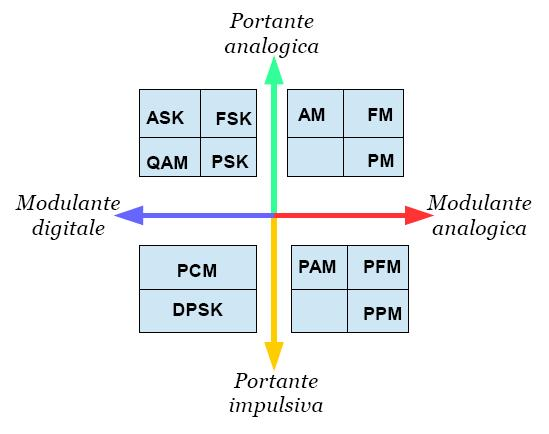
\includegraphics[scale = 1]{classificazione_modulazioni.jpg}
\end{figure}

\newpage 

\section{Rappresentazioni di segnali in modulazione}
\footnote{Slide del prof | Modulazioni analogiche | pag 1 - 2 \\  
Appunti di Damiano| pag 1 - 2 \\
Appunti | Modulazioni analogiche | pag 1 - 2 \\
Appunti | 2025-02-28 | pag 2
} 

Un significativo esempio di applicazione della Teoria dei Segnali, si rinviene nella rappresentazione 
nel dominio del tempo e della frequenza dei segnali modulati. \newline 

Nell'ambito delle telecomunicazioni, il termine modulazione sta ad indicare l'operazione (o in generale, il complesso delle operazioni) 
che consente di trasferire l'informazione da trasmettere (chiamato segnale modulante) in uno o più parametri di un segnale di portante. \newline 

Il risultato di questo "trasferimento" è un nuovo segnale chiamato segnale modulato. \newline 

Possiamo schematizzare la modulazione in questa maniera: 

\begin{figure}[h]
    \centering
    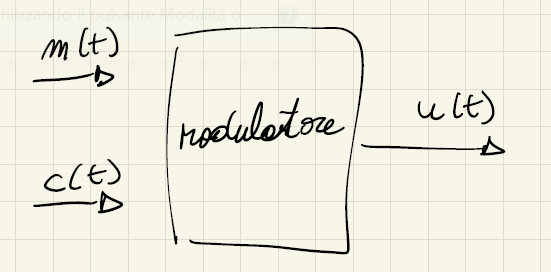
\includegraphics[scale = 0.5]{Schema della modulazione.PNG}
\end{figure}

dove: 

\begin{itemize}
    \item  m(t) è il segnale modulante, dall'inglese modulating signal 
    \item c(t) è il segnale portante, dall'inglese carrier
    \item u(t) è il segnale modulato
\end{itemize}

Il segnale modulato è quello più idoneo alla trasmissione nel canale e può essere inviato nel canale con le modalità che si sono scelte a priori. \newline

Benché la modulazione possa essere riferita anche a segnali passa-basso (ad esempio nel mixer di uno strumento musicale), 
"storicamente" la modulazione nasce per trasformare segnali passa-basso (cioè in banda base) in segnali passa-banda (quindi che dalla banda base li troveremo in alta frequenza, i.e. traslati nello spettro). \newline 

Questa traslazione in frequenza è dovuta principalmente a tre punti: 

\begin{enumerate}
    \item Necessità di utilizzare antenne di dimensioni ridotte nelle trasmissioni radio: la frequenza di trasmissione dipende dalla lunghezza d'onda del segnale, che deve essere uguale alle dimensioni dell'antenna 
    \item Necessità di utilizzare al meglio la funzione di trasferimento del canale trasmissivo: la modulazione permette di modulare il segnale modulante, che si trova in BB (Banda Base) in intervalli di frequenze in cui il canale distorce meno il segnale 
    \item Necessità di trasmettere contemporaneamente più segnali che originariamente occupano lo stesso intervallo di frequenze: si pensi ad esempio al segnale musicale in BB che deve essere trasmesso nella radio commerciale 
\end{enumerate}

\begin{tcolorbox}
    È vero che adesso esistono i podcast, ma ricordati di ascoltare un po' la radio. \newline 

    Prima di diventare anche tu zanzaroso e accendere la radio per ascoltare La Zanzara con David Parenzo e Cruciani, 
    ascoltati altri programmi interessanti nel palinsesto della "Radio di Confindustria". \newline 
    
    Te ne consiglio due dal lunedì al venerdì: 
    \begin{itemize}
        \item Due di Denari, con Mauro Meazza e Debora Rosciani, dalle 11 alle 12 \\ \url{https://www.radio24.ilsole24ore.com/conduttori/debora-rosciani/programmi/due-denari} 
        \item Focus economia, con Sebastiano Barisoni, dalle 17 alle 18:30, specialmente l'immancabile episodio di venerdì con la "poco invidiabile classifica degli sprechi" \\ \url{https://www.radio24.ilsole24ore.com/programmi/focus-economia} 
    \end{itemize}

    Prima il dovere e poi il piacere. \newline 

    AVANTI TIGRE
\end{tcolorbox}

Oltre ai vantaggi appena elencati, ce ne sono molti altri che non stiamo qui ad elencare. \newline 

Un grosso vantaggio della modulazione è l'allargamento dello spettro, che permette di migliorare l'immunità della trasmissione ai diversi agenti di disturbi di norma presenti. \newline 

Generalmente il disturbo principale che avremo a che fare è il nostro "caro amico" rumore termico. \newline 

\begin{tcolorbox}
   Al nostro caro amico rumore termico gli dedico questa canzone: \newline
   
   Toy Story - Un amico in me \\
   \url{https://youtu.be/0O_WONxv5p0?si=Hp4Aiu4OBY5xu6pT}
\end{tcolorbox}

\newpage 

\section{Modulazione analogica di una portante sinusoidale}
\footnote{Slide del prof | Modulazioni analogiche | pag 3 \\  
Appunti di Damiano| pag 3 \\
Appunti | Modulazioni analogiche | pag 3 \\
Appunti | 2025-02-28 | pag 3
} 

Un segnale c(t) (carrier, cioè segnale di portante) sinusoidale può essere descritto dalla seguente equazione: 

{
    \Large 
    \begin{equation}
        c(t) = A_c \cdot \cos(2 \pi f_c t + \phi_c)
    \end{equation}
}

dove: 

\begin{itemize}
    \item $A_c$ è l'ampiezza della sinusoide 
    \item $f_c$ è la frequenza, cioè l'inverso del periodo T di una sinusoide 
    \item t è il tempo 
    \item $\phi_c$ è la fase iniziale
\end{itemize}

Da un punto di vista grafico, nel tempo t possiamo visualizzare i parametri della sinusoide con la seguente figura: 

\begin{figure}[h]
    \centering
    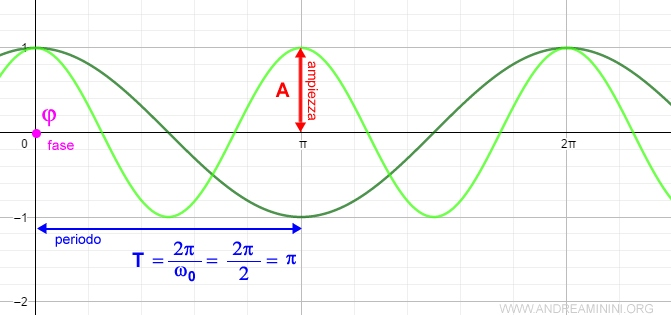
\includegraphics[scale = 0.5]{segnale-sinusoidale-aumento-freq.jpg}
\end{figure}

oppure nel piano fasoriale (che ci sarà molto utile nelle future trattazioni): 

\begin{figure}[h]
    \centering
    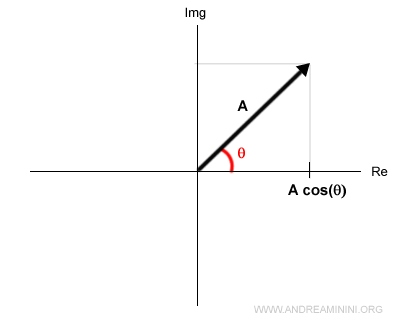
\includegraphics[scale = 0.5]{fasore-esempio-sinusoide.jpg}
\end{figure}

dove: 

\begin{itemize}
    \item $A \cdot \cos(\theta)$ è la proiezione del vettore $\overrightarrow{A}$ sull'asse reale 
    \item $A \cdot \sin(\theta)$ è la proiezione del vettore $\overrightarrow{A}$ sull'asse immaginario 
\end{itemize}

\newpage

Con la seguente figura: 

\begin{figure}[h]
    \centering
    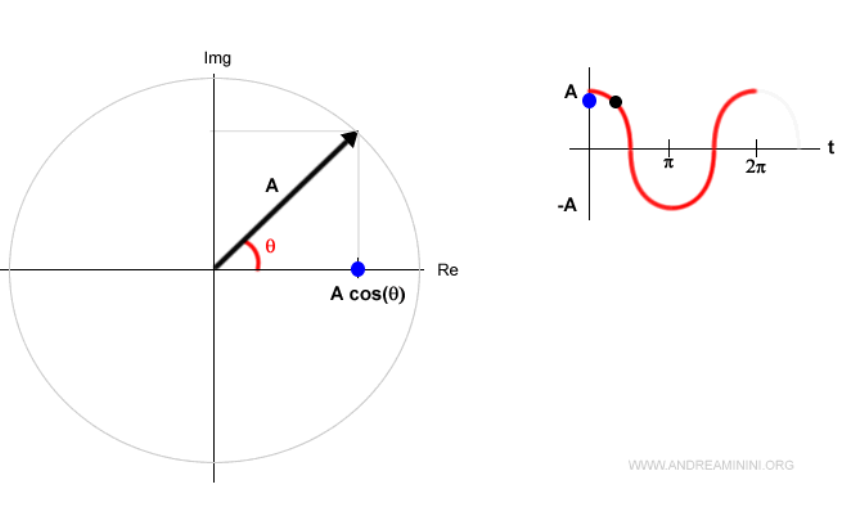
\includegraphics[scale = 0.5]{Piano fasoriale e andamento nel tempo.PNG}
\end{figure}

possiamo capire la relazione tra l'andamento nella sinusoide nel tempo e il piano fasoriale. \newline 

\begin{tcolorbox}
    Sembra banale ripassare i concetti basilari di una sinusoide, ma meglio essere tutti sulla stesso punto di inizio che far finta di capire qualcosa. \newline 
    
    Per approfondire: \\
    \url{https://www.andreaminini.org/telecomunicazioni/il-segnale-sinusoidale}
\end{tcolorbox}

Ritornando alla formula di c(t): 

{
    \Large 
    \begin{equation}
        c(t) = A_c \cdot \cos(2 \pi f_c t + \phi_c)
    \end{equation}
}

è evidente che è caratterizzata da tre gradi di libertà (cioè parametri che possiamo cambiare): 

\begin{itemize}
    \item l'ampiezza $A_c$ 
    \item la frequenza $f_c$ 
    \item la fase iniziale $\theta_c$
\end{itemize}

\begin{tcolorbox}
    Rispetto al corso di Segnali Determinati e Aleatori, o Teoria dei segnali per quelli del vecchio ordinamento, 
    in questo corso si predilige l'uso della frequenza f piuttosto che dei radianti $\omega$. \newline
    
    La relazione tra radianti e frequenza è la seguente: 

    {
        \Large 
        \begin{equation}
            \omega = 2 \pi f
        \end{equation}

    }
    
\end{tcolorbox} 


Questi gradi di libertà sono costanti e invariabili per qualunque istante di tempo nel segnale c(t). \newline 

Con la modulazione si vuole far dipendere uno o più di questi parametri di c(t), detto segnale di portante, a dei parametri di un altro segnale m(t), 
detto appunto segnale modulante. \newline 

Si parlerà di: 

\begin{itemize}
    \item modulazione di ampiezza (Amplitude Modulation o AM) quando l'ampiezza $A_c$ verrà resa dipendente da m(t)
    \item modulazione in frequenza (Frequency Modulation o FM) quando la frequenza $f_c$ verrà resa dipendente da m(t)
    \item modulazione di fase (Phase Modulation o PM) quando la fase iniziale $\phi_c$ verrà resa dipendente da m(t)
\end{itemize}

In realtà, si avrà modo di precisare che sia la modulazione di frequenza e sia la modulazione di fase sono tra loro intimamente legate: 
per cui, ove si realizzi una modulazione di frequenza, si realizza anche una modulazione di fase e viceversa. \newline 

Per questo motivo, sia la modulazione di fase che di frequenza, possono essere definite anche come modulazioni angolari, 
perché il segnale modulante agisce sull'angolo della funzione sinusoide. \newline 

\newpage 

\section{Modulazione di ampiezza}
\footnote{Slide del prof | Modulazioni analogiche | pag 3 \\  
Appunti di Damiano| pag 3 \\
Appunti | Modulazioni analogiche | pag 3 \\
Appunti | 2025-02-28 | pag 3
} 

Ritornando al segnale c(t): 

{
    \Large 
    \begin{equation}
        c(t) = A_c \cdot \cos(2 \pi f_c t + \phi_c)
    \end{equation}
}

andiamo a spiegare diverse modulazioni in cui l'ampiezza $A_c$ verrà resa dipendente da m(t), segnale modulante. \newline 

\newpage 

\subsection{Banda Laterale Doppia Portante Soppressa (DSB-SC)}
\footnote{Slide del prof | Modulazioni analogiche | pag 3 - 6\\  
Appunti di Damiano| pag 3 - 6\\
Appunti | Modulazioni analogiche | pag 3 - 6 \\
Appunti | 2025-02-28 | pag 3 - 5 \\
Appunti | 2025-03-03 | pag 2
} 

Nella modulazione di ampiezza con banda laterale doppia portante soppressa (o più frequentemente DSB-SC: Double Side Band - Suppressed Carrier), 
il segnale modulato u(t) è ottenuto semplicemente moltiplicando il segnale c(t) per il segnale modulante m(t). \newline 

In formula: 

{
    \Large 
    \begin{equation}
        \begin{split}
            u (t) 
            &= 
            m(t) \cdot c(t)
            \\
            &=
            m(t) \cdot \left[ A_c \cdot \cos(2 \pi f_c t + \phi_c) \right]
            \\
            &= 
            \left[A_c \cdot m(t) \right] \cdot \cos(2 \pi f_c t + \phi_c)
        \end{split}
    \end{equation}
}

Un esempio si segnale modulato u(t): 

{
    \Large 
    \begin{equation}
        u (t) 
        = 
        \left[A_c \cdot m(t) \right] \cdot \cos(2 \pi f_c t + \phi_c)
    \end{equation}
}

partendo da un segnale m(t) modulante è raffigurato nelle seguenti figure: 

\begin{figure}[h]
    \centering
    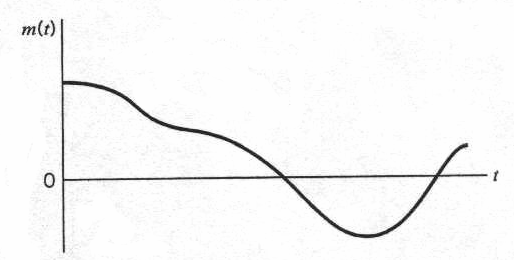
\includegraphics[scale = 0.8]{Segnale modulante.png}
    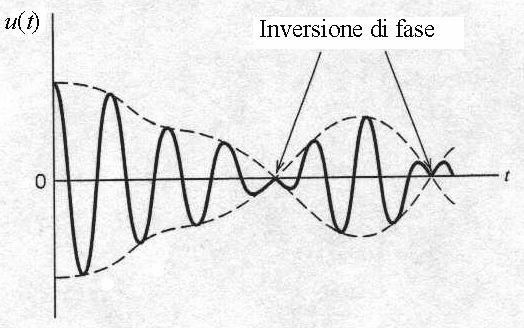
\includegraphics[scale = 0.8]{Segnale modulato in AM.png}
\end{figure}

È interessante l'inversione di fase del segnale modulato in corrispondenza dei passaggi per lo zero del segnale modulante. \newline 

Inoltre, nella figura di u(t), è tratteggiato l'andamento di m(t). \newline 

Utilizzando le proprietà della trasformata di Fourier, cioè quella della trasformazione in frequenza e quella del prodotto,
u(t) ha una semplice rappresentazione in frequenza: 

{
    \Large 
    \begin{equation}
        \begin{split}
        u (t) 
        &= 
        \left[A_c \cdot m(t) \right] \cdot \cos(2 \pi f_c t + \phi_c)
        \\
        &\downarrow
        \\
        U(f)
        &=
        \frac{A_c}{2}
        \left[
            M (f - f_c) e^{\jmath \theta_c}
            +
            M (f + f_c) e^{-\jmath \theta_c}
        \right]
        \end{split}
    \end{equation}
}


\begin{tcolorbox}
    
    Da \url{https://github.com/ciccio25/appunti-teoria-dei-segnali/blob/main/Appunti%20Teoria%20dei%20segnali.pdf} \\
    Capitolo 3.3 Proprietà della trasformata di Fourier | pag 22 - 23 \newline
    
    \textbf{Proprietà della traslazione in frequenza}

Considerando $\omega_1$ la frequenza traslata, possiamo dire che: 

{
    \Large 
    \begin{equation}
        s^{'} (t) = s(t) e^{\jmath \omega_1 t} 
        \leftrightarrow 
        S^{'} (\omega) = S(\omega -\omega_1)
    \end{equation}
}

\textbf{Proprietà del prodotto}

{
    \Large 
    \begin{equation}
        s^{'} (t) = s_1(t) s_2 (t) 
        \leftrightarrow 
        S^{'}(\omega) = \frac{1}{2 \pi} \int_{-\infty}^{\infty}S_1(\theta) S_2 (\omega - \theta) d\theta
    \end{equation}
}

L'integrazione viene svolta su $\theta$ e $\omega$ viene visto come parametro nella formula di integrazione. \newline 

$\blacksquare$ \newline 

Da \url{https://www.andreaminini.org/telecomunicazioni/il-fasore} \newline

$e^{-\jmath \theta_c}$ è un $\cos(\omega t + \theta_c)$ nell'asse dei tempi 

\end{tcolorbox}

In frequenza i segnali m(t) e u(t) possiamo rappresentarli come in figura: 

\begin{figure}[h]
    \centering
    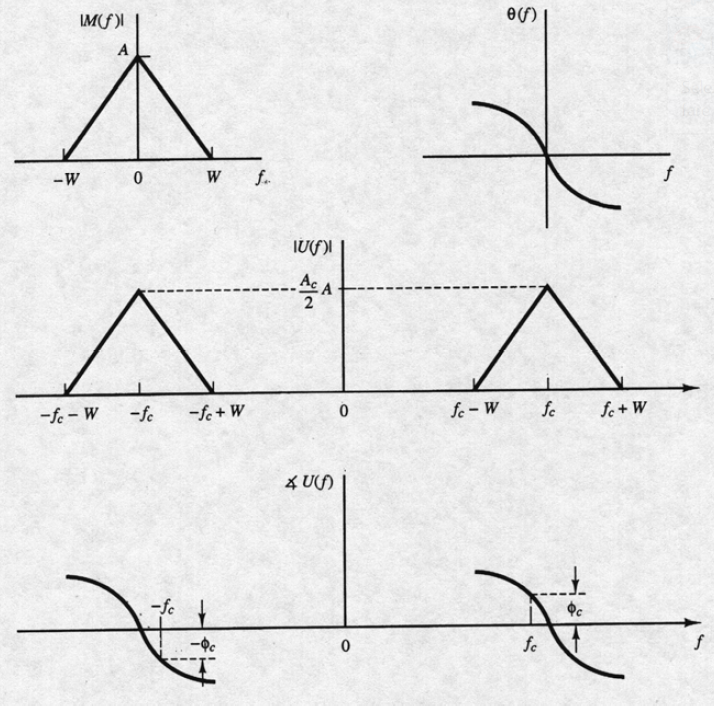
\includegraphics[scale = 1]{Segnale modulato e modulante in AM.PNG}
\end{figure} 

Questa figura mette in evidenzia tutte le caratteristiche peculiari della modulazione DSB-SC. \newline 

La modulazione trasla lo spettro del segnale di $\abs{M(f)}$ da $[-W, +W]$ a $\abs{U(f)}$ in $[-f_c - W, -f_c +W]$ e $[f_c - W, f_c +W]$. \newline 

Il modulo di $\abs{M(f)}$ in $\abs{U(f)}$ resta inalterato (a meno di un fattore moltiplicativo che è $\frac{A_c}{2}$). \newline 

L'unico parametro che cambia è quello della fase che passa da $\theta(f) = 0$ in f a $-\theta_c$ a $-f_c$ e $\theta_c$ a $f_c$. \newline 

In altre parole, la fase iniziale viene incrementata di $\theta_c$ nelle frequenze positive e viene ridotta di $\theta_c$ per quanto riguarda le frequenze negative. \newline 

A meno di questo sfasamento (che peraltro è nullo quando $\theta_c = 0$), 
lo spettro del segnale non viene modificato dalla modulazione. \newline 

Per questo motivo, la modulazione DSB-SC, e più in generale la modulazione in ampiezza, 
viene classificata come "lineare" anche se non è una modulazione svolta con componenti lineari. \newline 

Un sistema lineare, può eliminare (cioè si comporta da filtro) o equalizzare (cioè svolge un equalizzatore di ampiezza o di fase) totalmente o in parte le frequenze che gli si presentano in ingresso, 
ma non ne potrà mai introdurre di nuove. \newline 

Dalla figura degli spettri del segnale modulato rispetto al segnale modulante, 
$M(f)$ occupa una banda $[-W, +W]$, invece $U(F)$ occupa $[-f_c - W, -f_c +W]$ e $[f_c - W, f_c +W]$, 
che è il doppio della banda occupata da M(f). \newline 

Prende il nome di banda laterale superiore di U(f) (o come è stato definito a lezione Banda Laterale Superiore BLSup) 
la parte dello spettro per $\abs{f} > f_c$. \newline 

Prende il nome di banda laterale inferiore di U(f) (o come è stato definito a lezione Banda Laterale Inferiore BLInf) 
la parte dello spettro per $\abs{f} < f_c$. \newline 

Il seguente schema ci può far capire meglio la differenza tra banda laterale superiore e banda laterale inferiore: 

\begin{figure}[h]
    \centering
    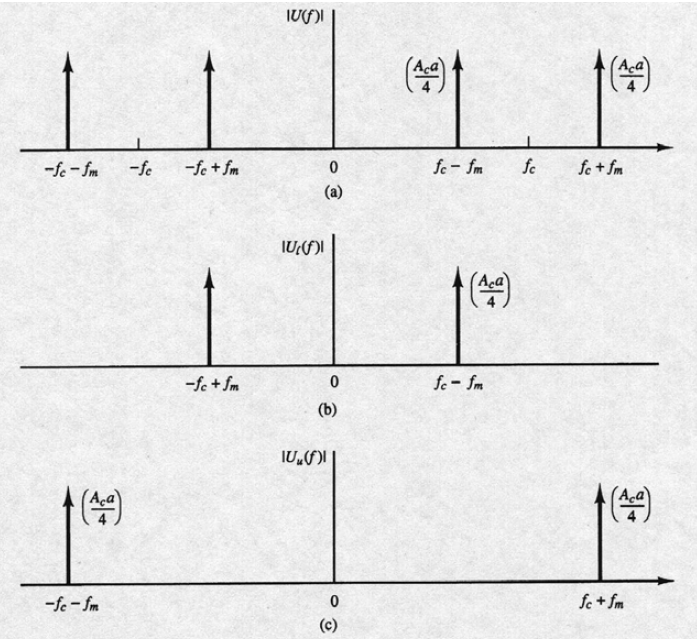
\includegraphics[scale = 1]{Bande laterali.PNG}
\end{figure} 

Se la modulante è sinusoidale, grazie alle proprietà di Fourier, avremo come segnale modulato una serie di righe nello spettro in frequenza (come si vede in figura da $\abs{U(f)}$). \newline 

$\abs{U_u (f)}$ è lo spettro della banda superiore (u dall'inglese si intende upper, superiore in italiano), 
$\abs{U_l (f)}$ è lo spettro della banda inferiore (l dall'inglese si intende lower, inferiore in italiano) 

Quindi, come si vede dalla figura, in $\abs{U_u (f)}$ ci sono solo le frequenze a $[-f_c + f_m]$ e $[f_c - f_m]$, 
in $\abs{U_l (f)}$ ci sono solo le frequenze a $[-f_c - f_m]$ e $[f_c + f_m]$. \newline 

Grazie al concetto dei processi stocastici, in particolare della teoria dei processi ciclo-stazionari, i segnali determinati e le loro proprietà si estendono anche ai segnali di spettro di potenza, 
cioè quelli che abbiamo visto in figura. \newline 

\begin{tcolorbox}
    
    Da \url{https://github.com/ciccio25/appunti-teoria-dei-segnali/blob/main/Appunti%20Teoria%20dei%20segnali.pdf} \\
    Capitolo 13 Processi stocastici | pag 151 - 160 \newline

\end{tcolorbox}

\newpage 

\subsubsection{Demodulazione per la DSB-SC}
\footnote{Slide del prof | Modulazioni analogiche | pag 6 - 8\\  
Appunti di Damiano| pag 6 - 8\\
Appunti | Modulazioni analogiche | pag 6 - 8 \\
Appunti | 2025-03-03 | pag 3 - 11
} 

Un ultimo aspetto riguarda la demodulazione, cioè la capacità di riottenere il segnale modulante a partire dal segnale modulato. \newline 

In un sistema di comunicazioni, la demodulazione avviene al lato ricevente quando si deve recuperare l'informazione m(t) per renderla utilizzabile dal destinatario. \newline 

Si pensi ad un segnale telefonico: la voce umana sta nella banda da 300 Hz a 3400 Hz. \newline 

Nella trasmissione sul canale, ad esempio il cavo di rame, il segnale voce viene modulato ad alta frequenza 
in modo da essere trasportato nella rete di telecomunicazioni, e alla fine viene ricevuto dal destinatario che riporta il segnale modulato in alta frequenza alla frequenza originale, 
così da poter ascoltare la voce del mittente. \newline 

In assenza di rumore, distorsione o altre cause di disturbo, 
il segnale ricevuto r(t) coincide con m(t): 
il modo concettuale per riottenere il segnale m(t) non è quello di dividere per la portante, 
bensì moltiplicare r(t) per un segnale sinusoidale. \newline 

Il segnale sinusoidale sarà proprio il segnale di portante, che è sta generata localmente dal ricevitore, 
con la stessa frequenza e con la stessa fase della portante ricevuta. \newline 

In formule, se si è ricevuto r(t) e grazie alle proprietà trigonometriche: 

{
    \Large 
    \begin{equation}
        \begin{split}
        r(t) \cdot \cos(2 \pi f_c t + \phi_c) 
        &=
        A_c \cos^{2}(2 \pi f_c t + \phi_c)
        \\
        &=
        A_c m(t) \cdot \frac{1 + \cos[2\cdot (2 \pi f_c t + \phi_c)]}{2} 
        \\
        &=
        \frac{1}{2} A_c m(t)
        +
        \frac{1}{2} A_c m(t)
        \cos[2\cdot (2 \pi f_c t + \phi_c)]
        \\
        &=
        \frac{1}{2} A_c m(t)
        +
        \frac{1}{2} A_c m(t)
        \cos(4 \pi f_c t + 2 \phi_c)
    \end{split}
    \end{equation}
}

\begin{tcolorbox}
    Ripasso delle formule trigonometriche che non fa mai male: \\
    \url{https://www.youmath.it/formulari/65-formulari-di-trigonometria-logaritmi-esponenziali/159-identita-trigonometriche-formule-di-prostaferesi-formule-di-werner.html} \newline 

    In questo corso le utilizzeremo spesso, quindi può essere comodo averle sempre sotto mano
\end{tcolorbox}

Osservando la formula appena scritta, possiamo fare le seguenti considerazioni: 

\begin{itemize}
    \item Aggiungendo un filtro passa basso con frequenza di taglio a $2 \pi f_c$, possiamo togliere tutta la componente in alta frequenza 
    \item $\frac{1}{2} A_c$ è solo un fattore moltiplicativo
\end{itemize}

Con queste osservazioni, possiamo semplificare l'equazione del demodulatore come: 

{
    \Large 
    \begin{equation}
        \begin{split}
        r(t) \cdot \cos(2 \pi f_c t + \phi_c) 
        &=
        \frac{1}{2} A_c m(t)
        +
        \frac{1}{2} A_c m(t)
        \cos(4 \pi f_c t + 2 \phi_c)  
        \\
        &\downarrow
        \\
        r(t) \cdot \cos(2 \pi f_c t + \phi_c)
        &= 
        \frac{1}{2} A_c m(t)
        \end{split}
    \end{equation}
}

Cioè il segnale ricevuto e de-modulato è proprio il segnale originale in banda base, a meno del fattore moltiplicativo $\frac{1}{2} A_c$. \newline 

Possiamo schematizzare il demodulatore con la seguente figura: 

\begin{figure}[h]
    \centering
    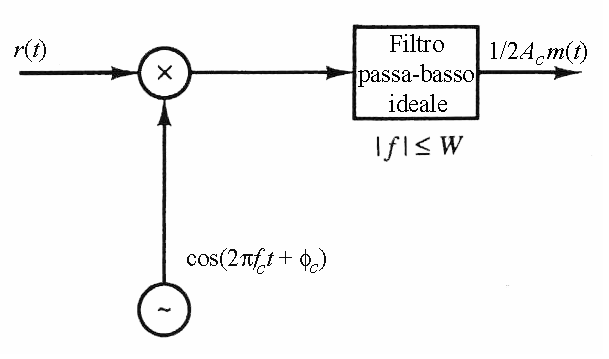
\includegraphics[scale = 1]{Schema architettura di un demodulatore.png}
\end{figure} 

Se invece consideriamo una differenza di fase tra la portante ricevuta e la portante generata localmente, 
avremo la seguente equazione: 

{
    \Large 
    \begin{equation}
            r(t) \cos(2 \pi f_c t + \phi)
            = 
            \frac{1}{2} A_c m(t) \cos(\phi_c - \phi)
            + 
            \frac{1}{2} A_c m(t) \cos(4 \pi f_c t + \phi_c - \phi)
    \end{equation}
}

A valle del filtro passa-basso del demodulatore, e per le considerazioni svolte precedentemente, avremo il segnale di uscita $y_l (t)$:

{
    \Large 
    \begin{equation}
        \begin{split}
            r(t) \cos(2 \pi f_c t + \phi)
            &= 
            \frac{1}{2} A_c m(t) \cos(\phi_c - \phi)
            + 
            \frac{1}{2} A_c m(t) \cos(4 \pi f_c t + \phi_c - \phi)
            \\
            &\downarrow
            \\
            y_l (t)
            &= 
            \frac{1}{2} A_c m(t) \cos(\phi_c - \phi)
        \end{split}
    \end{equation}
}

Questa ultima espressione di $y_l (t)$ mette in evidenzia che, rispetto al caso ideale: 

{
    \Large 
    \begin{equation}
        y_l^{'} (t) = \frac{1}{2} A_c m(t)
    \end{equation}
}

il segnale utile in uscita è ridotto del fattore $\cos(\theta_c - \theta)$. \newline 

Se: 

{
    \Large 
    \begin{equation}
        \theta_c - \theta = 90 ^{\circ}
    \end{equation}
}

$y_l (t)$ diventa: 

{
    \Large 
    \begin{equation}
       \begin{split}
        y_l (t)
            &= 
            \frac{1}{2} A_c m(t) \cos(\phi_c - c)
            \\
            &\downarrow
            \\
            y_l (t)
            &= 
            \frac{1}{2} A_c m(t) \cos(90 ^{\circ})
            \\
            &= 
            \frac{1}{2} A_c m(t) \cdot 0 
            \\
            &= 
            0
       \end{split} 
    \end{equation}
}

cioè $y_l (t)$ si annulla. \newline 

In caso di un segnale utile sovrapposto ad un contributo di rumore (ad esempio il rumore termico), 
la rivelazione imperfetta riduce la potenza del segnale utile, rendendo quest'ultimo più vulnerabile agli effetti del rumore. \newline 

Il demodulatore raffigurato precedentemente è detto anche ricevitore sincrono (o coerente). \newline 

Viene definito ricevitore coerente perché, per ricavare il segnale modulante, 
si moltiplica il segnale modulato per un coseno. \newline  

Il problema della ricostruzione della fase $\theta_c$ della portante è uno dei problemi di maggior importanza nell'ambito della ricezione sincrona e viene tipicamente risolto con i PLL (Phase-Locked Loop). \newline 

In alternativa, la demodulazione può essere semplificata sovrapponendo alla trasmissione del segnale DSB-SC la trasmissione di un residuo di portante, 
utilizzando il seguente schema: 

\begin{figure}[h]
    \centering
    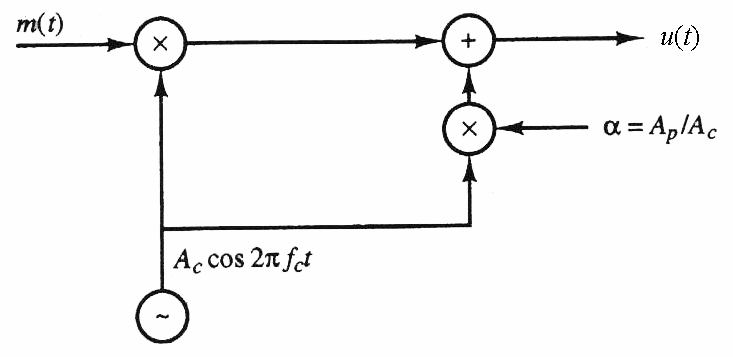
\includegraphics[scale = 1]{Modulazione DSB-SC con resudio di portante.png}
\end{figure} 

Rispetto al caso precedente, u(t) sarà: 

{
    \Large 
    \begin{equation}
        u (t)
        = 
        \left[A_c m(t) + \frac{A_p}{A_c} \right] \cdot \cos(2 \pi f_c t)
    \end{equation}
}

dove $A_p$ viene definito come residuo di portante, la cui ampiezza è una frazione di $\alpha$ di $A_c$: 
$A_c$ viene definito come tono pilota. \newline 

\newpage 

In frequenza avremo: 

\begin{figure}[h]
    \centering
    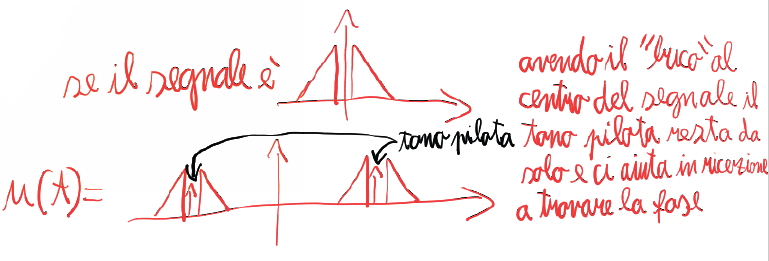
\includegraphics[scale = 1]{Aggiunta del tono pilota DSB-SC.PNG}
\end{figure} 

Con questo schema non vi è necessità di generare localmente la portante al ricevitore, 
ma il prezzo che si paga è in termini di potenza trasmessa addizionale e di intervallo di frequenza non utilizzabile 
perché necessario alla trasmissione della portante. \newline 

In questo senso, rispetto al caso senza tono pilota, lo schema DSB-SC costituisce una soluzione "ibrida", 
che permette di avere un demodulatore più semplice ed a costo economico ridotto, ma sprecando nettamente più energia in trasmissione. \newline 

\newpage 

\subsection{Modulazione di ampiezza convenzionale - AM}
\footnote{Slide del prof | Modulazioni analogiche | pag 8 - 11\\  
Appunti di Damiano| pag 8 - 11\\
Appunti | Modulazioni analogiche | pag 8 - 11\\
Appunti | 2025-03-03 | pag 11 - 13
}

Nella sezione precedente, cioè riguardo alla DSB-SC, abbiamo discusso e analizzato una DSB-SC con una portante quando si va in trasmissione per semplificare il ricevitore: 
questo caso particolare è proprio la tecnica AM (Amplitude Modulation) convenzionale della modulazione DSB-SC. \newline 

Riportando lo schema del modulatore AM: 

\begin{figure}[h]
    \centering
    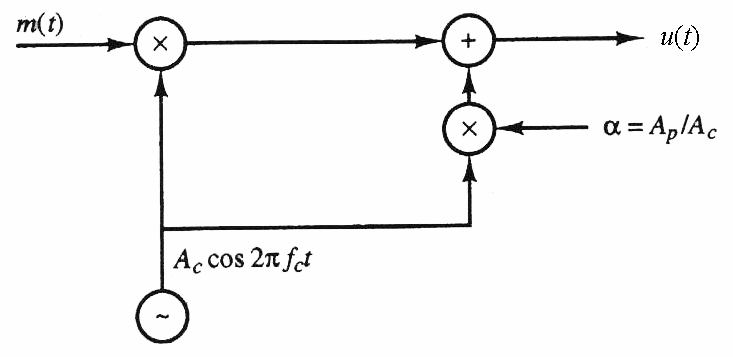
\includegraphics[scale = 1]{Modulazione DSB-SC con resudio di portante.png}
\end{figure} 

il segnale modulato in uscita u(t) sarà: 

{
    \Large 
    \begin{equation}
        u (t)
        = 
        A_c 
        [1 + \alpha \cdot m_n (t)] 
        \cos(2 \pi f_c t + \phi_c)
    \end{equation}
}

dove: 

{
    \Large 
    \begin{equation}
        \begin{cases}
            m_n(t) = \frac{m(t)}{\max \abs{m(t)}}
            \\
            0 < \alpha \le 1
        \end{cases}    
    \end{equation}
}

$m_n (t)$ è definito come "segnale modulante normalizzato", 
invece $\alpha$ è definito come "indice di modulazione di ampiezza". \newline 

Grazie alle definizioni di $m_n (t)$ e $\alpha$, possiamo dire che u(t) non diventa mai negativa nel tempo. \newline 

Considerando il caso particolare in cui:

{
    \Large 
    \begin{equation}
        \begin{cases}
            m_n(t_0) = - 1 
            \\
            \alpha = 1
        \end{cases}
    \end{equation}
}

\newpage 

l'andamento del segnale modulato u(t) è il seguente: 

\begin{figure}[h]
    \centering
    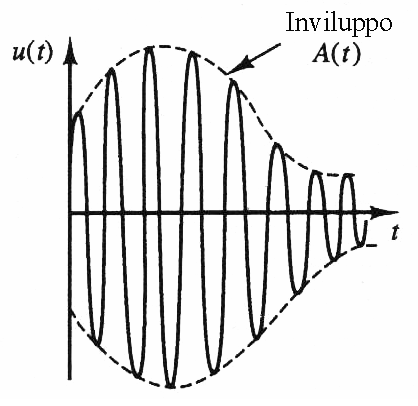
\includegraphics[scale = 1]{Segnale modulato AM con alpha a 1.png}
\end{figure} 

e confrontando il segnale modulato in AM con quello a DSB-SC: 

\begin{figure}[h]
    \centering
    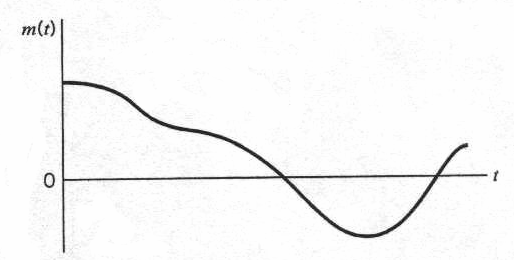
\includegraphics[scale = 0.8]{Segnale modulante.png}
    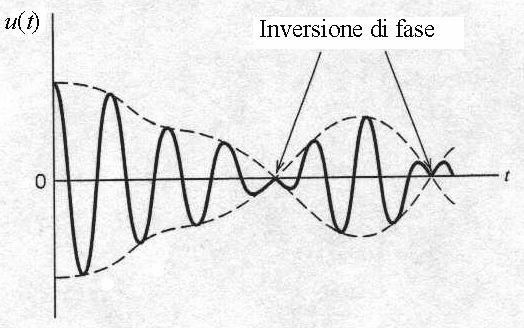
\includegraphics[scale = 0.8]{Segnale modulato in AM.png}
\end{figure}

notiamo che in AM, l'inviluppo mantiene l'andamento del segnale modulante (cioè quello tratteggiato in figura): 
è proprio per questa caratteristica che la demodulazione del segnale AM convenzionale può essere particolarmente semplice. \newline 

Inoltre, nei passaggi sullo zero, in AM non ci sono inversioni della fase. \newline 

Per inviluppo si intende che la sequenza dei massimi tra segnale modulato e modulante è la stessa. \newline 

La trasformata di Fourier di un segnale in AM convenzionale diventa: 

{
    \Large 
    \begin{equation}
        \begin{split}
        u (t)
        &= 
        A_c 
        [1 + \alpha \cdot m_n (t)] 
        \cos(2 \pi f_c t + \phi_c)
        \\
        &\quad
        \\
        &\downarrow
        \\
        &\quad
        \\
        U(f)
        &= 
        \frac{A_c}{2}
        \left[
            e^{\jmath \phi_c} a M_n (f - f_c)
            +
            e^{\jmath \phi_c} \delta (f - f_c)
            +
            e^{-\jmath \phi_c} a M_n (f + f_c)
            +
            e^{-\jmath \phi_c} \delta (f + f_c)
        \right]
    \end{split}
    \end{equation}
}

dove $M_n (f)$ è la trasformata di Fourier del segnale modulante normalizzato. \newline 

\newpage 

Un esempio di andamento di U(f), nel caso di modulante sinusoidale, è mostrato nella seguente figura: 

\begin{figure}[h]
    \centering
    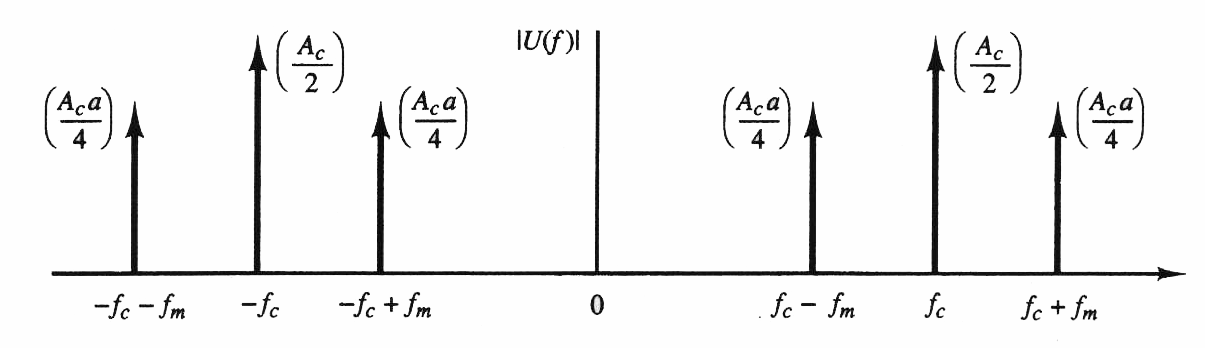
\includegraphics[scale = 0.6]{Segnale modulato in AM in frequenza.png}
\end{figure} 

Rispetto allo spettro in frequenza di un segnale modulato in DSB-SC: 

\begin{figure}[h]
    \centering
    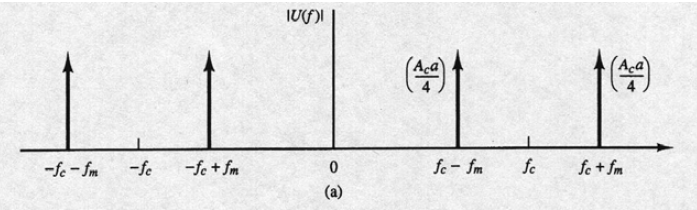
\includegraphics[scale = 1]{Segnale modulato in DSB-SC.PNG}
\end{figure} 

notiamo che, in AM convenzionale, è presente la portante a $\abs{f_c}$. \newline

Inoltre, si nota dalla figura, che, se ci troviamo nel caso di $\alpha = 1$, 
l'ampiezza della portante resta doppia di quella di ciascuno dei segnali assegnati alle bande laterali (in questo caso particolare, a loro volta sinusoidali). \newline 

Di conseguenza, anche nel caso limite di modulazione al 100 \%, cioè $\alpha = 1$, 
i $\frac{2}{3}$ della potenza complessiva del segnale modulato sono associati alla portante 
e solo la frazione rimanente, cioè $\frac{1}{3}$ è associata alla bande laterali. \newline 

Con valori di $\alpha < 1$, questo "squilibrio" si enfatizza, specialmente nei casi in cui $\alpha < \frac{1}{2}$, 
che sono la grande maggioranza dei segnali di interesse. \newline 

Il fatto di usare la maggior parte dell'energia di un segnale modulato per la portante è molto inefficiente dal punto di vista energetico, 
ma è molto utile per realizzare un circuito di demodulazione molto semplice. \newline 

Essendo l'informazione contenuta nell'inviluppo del segnale, 
è sufficiente ricostruire al ricevitore proprio l'inviluppo. \newline 

Quindi non è necessario un ricevitore coerente come nella DSB-SC (anche se tecnicamente lo si potrebbe utilizzare), 
ma possiamo utilizzare questo semplice circuito del demodulatore a inviluppo: 

\begin{figure}[h]
    \centering
    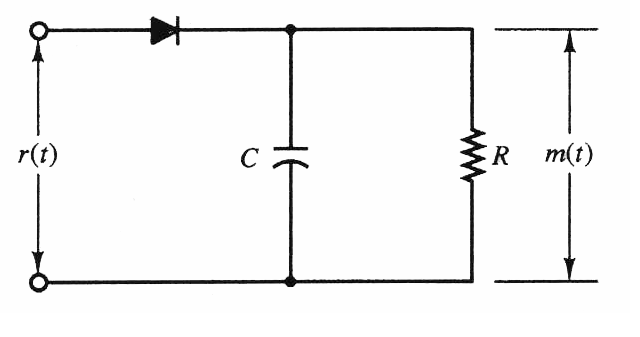
\includegraphics[scale = 1]{Demodulatore di inviluppo.png}
\end{figure} 

Questo demodulatore si definisce non coerente perché non si moltiplica r(t) per un coseno. \newline 

I componenti di questo demodulatore sono i seguenti: 

\begin{itemize}
    \item diodo, che è un componente non lineare che elimina le componenti r(t) quando quest'ultima diventa negativa 
    \item una capacità C 
    \item un resistore R
\end{itemize}

Attraverso una scelta adeguata dei componenti R-C (che realizzano un filtraggio passa-basso), 
si ottiene un andamento del segnale come la seguente figura: 

\begin{figure}[h]
    \centering
    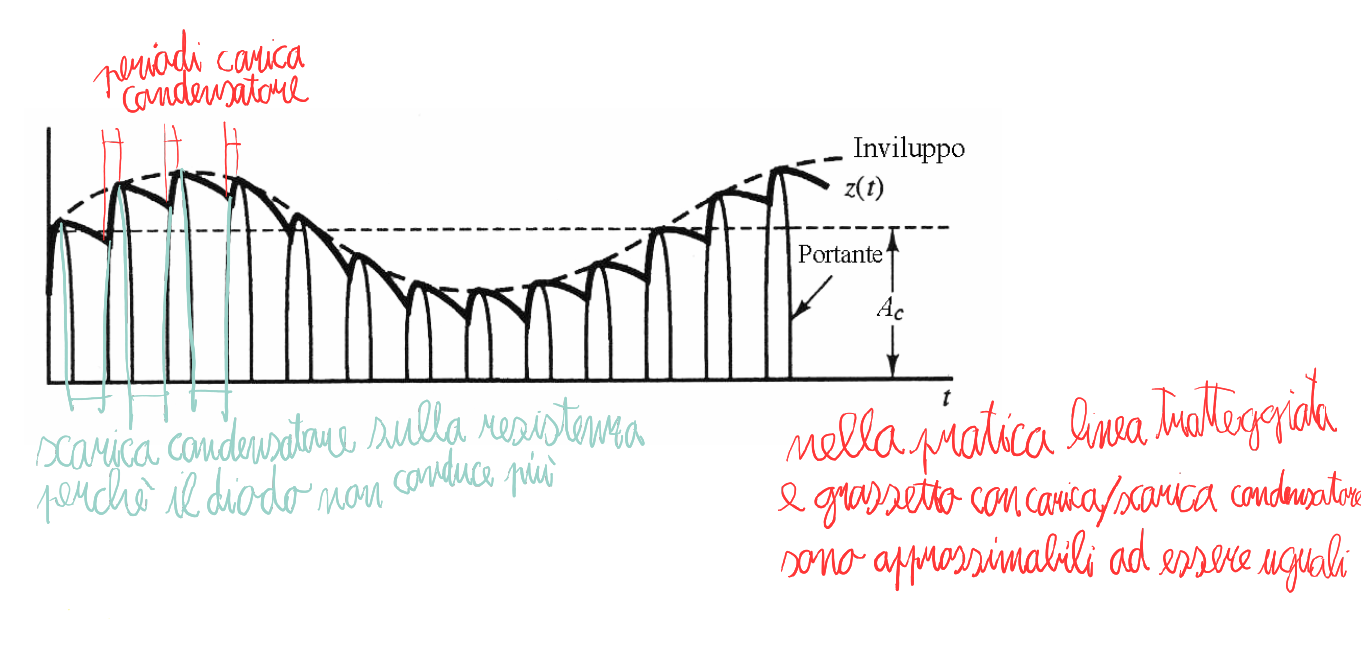
\includegraphics[scale = 0.65]{Segnale demodulato in AM con demodulatore a inviluppo.PNG}
\end{figure} 

La scelta di semplificare il ricevitore è decisiva in tutte quelle applicazioni in cui il numero dei trasmettitori è ridotto, 
mentre è elevato il numero dei ricevitori. \newline 

Per questo motivo l'utilizzo della AM convenzionale, o altre tecniche simili,
ha costituito la soluzione privilegiata (negli anni precedenti prima dell'avvento del digitale e dei componenti a basso costo)
per i servizi commerciali di tipo diffusivo come radio e televisione. \newline 

\newpage 

\subsection{Banda Laterale Unica (SSB)}
\footnote{Slide del prof | Modulazioni analogiche | pag 11 - 13\\  
Appunti di Damiano| pag 11 - 13\\
Appunti | Modulazioni analogiche | pag 11 - 13\\
Appunti | 2025-03-03 | pag 13
} 

L'obbiettivo della modulazione di ampiezza a banda laterale unica (acronimo italiano BLU o, in inglese SSB Single Side Band) 
è quello di migliorare l'efficienza spettrale. \newline 

Nelle tecniche precedenti trattate, cioè DSB-SC e AM convenzionale, 
la banda occupata dal segnale modulato era doppia rispetto a quella del segnale modulante. \newline 

Osservando alla forma dello spettro del segnale modulato, ad esempio quello in DSB-SC, e al modo in cui è stato ottenuto per traslazione dello spettro della banda base: 

\begin{figure}[h]
    \centering
    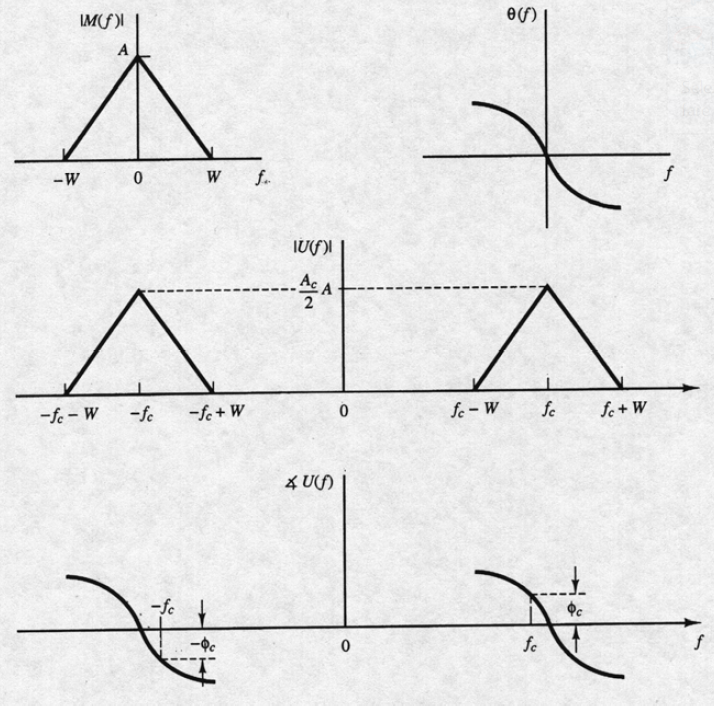
\includegraphics[scale = 0.7]{Segnale modulato e modulante in AM.PNG}
\end{figure} 

ci si convince facilmente che la ricostruzione del segnale è possibile anche conoscendo soltanto una delle due bande laterali. \newline 

L'andamento temporale del segnale SSB è del tipo: 

{
    \Large 
    \begin{equation}
        u(t)
        =
        A_c m(t) \cos(2 \pi f_c t)
        \mp
        A_c \tilde{m}(t) \sin(2 \pi f_c t)
    \end{equation}
}

dove $\tilde{m}(t)$ è la trasformata di Hilbert del segnale modulante. \newline 

\begin{tcolorbox}
    Come al solito, un altro argomento che abbiamo incontrato e studiato al precedente corso. \newline 

    Da \url{https://github.com/ciccio25/appunti-teoria-dei-segnali/blob/main/Appunti%20Teoria%20dei%20segnali.pdf} \\
    Capitolo 8 Trasformata di Hilbert | pag 83 - 85 \newline

\end{tcolorbox}

Per semplicità, si è trascurata la fase iniziale della portante $\phi_c$. \newline 

Nella formula è presente un segno $\mp$ perché si utilizza uno dei due casi: 

\begin{itemize}
    \item il segno negativo - se si è deciso di trasmettere la banda laterale superiore 
    \item il segno positivo + se si è deciso di trasmettere la banda laterale inferiore 
\end{itemize}

\newpage

Dalla formula di u(t) possiamo ricavare uno schema a blocchi del modulatore, che è il seguente: 

\begin{figure}[h]
    \centering
    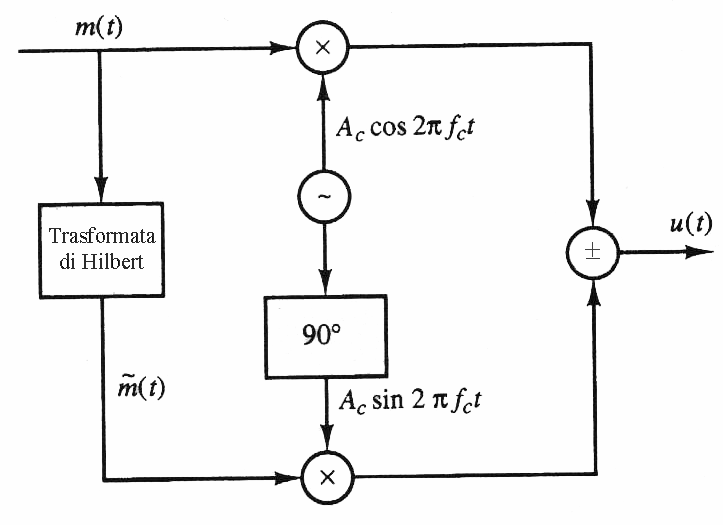
\includegraphics[scale = 0.7]{Modulazioone segnale SSB.png}
\end{figure}

Dalle proprietà della trasformata di Hilbert, ricordiamo che m(t) 
non deve avere un contenuto significativo alle basse frequenze, perché altrimenti si perderà informazione. \newline 

In alternativa, la stessa modulazione SSB può essere applicata con il seguente schema: 

\begin{figure}[h]
    \centering
    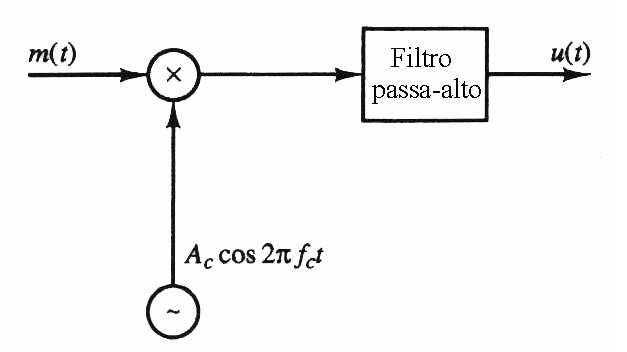
\includegraphics[scale = 0.7]{Modulazioone segnale SSB con filtro passa alto e DSB-SC.png}
\end{figure}

dove è presente un filtro passa-alto, con frequenza di taglio in prossimità della frequenza di portante $f_c$, 
del segnale m(t) modulato in DSB-SC.\newline 

\newpage 

Un esempio di spettro di segnale SSB, nel caso di segnale modulante stocastico è riportato nella seguente figura: 

\begin{figure}[h]
    \centering
    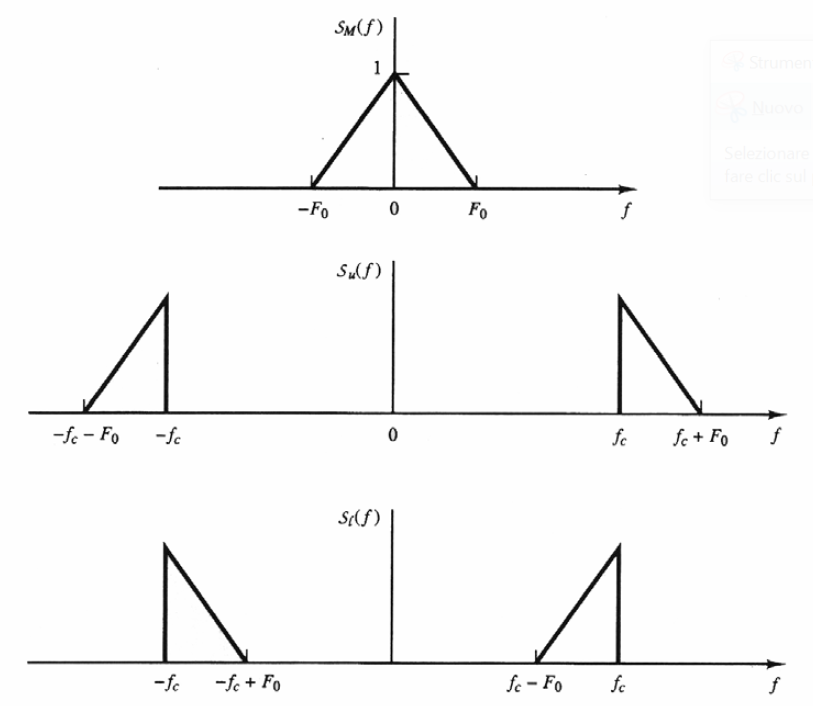
\includegraphics[scale = 0.7]{Spettri di potenza di un segnale in BB e SSB.PNG}
\end{figure}

dove: 

\begin{itemize}
    \item $S_M (f)$ è il segnale modulante in Banda Base 
    \item $S_u (f)$ è il segnale modulato in SSB con banda laterale superiore 
    \item $S_l (f)$ è il segnale modulato in SSB con banda laterale inferiore
\end{itemize}

Sapendo che il segnale modulante $S_M (f)$ si estende in banda da $[- F_0, +F_0]$, 
trasmettendo solo in banda superiore o solo in basa superiore, si occupa la metà della banda rispetto alla DSB-SC e la AM-convenzionale, 
mantenendo la stessa qualità. \newline 

O se si applica il filtraggio passa-alto dalla modulazione della DSB-SC o si utilizza il metodo con la trasformata di Hilbert, 
la SSB è assente di componenti significativi intorno alla frequenza d'origine. \newline 

Se infatti idealmente il filtraggio di Hilbert o quello passa-banda può avvenire con transizione brusca (o a frequenza nulla per la trasformata di Hilbert o a $f_c$ per il filtro passa-alto), 
come si può visualizzare nel seguente andamento del filtro di Hilbert: 

\begin{figure}[h]
    \centering
    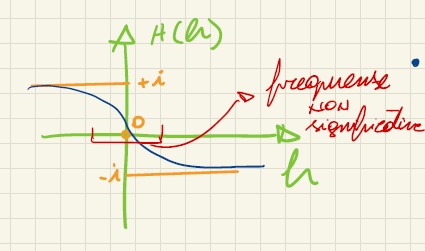
\includegraphics[scale = 0.5]{Considerazioni filtro di Hilbert in frequenza.PNG}
\end{figure} 

nella pratica un filtro reale presenterà una regione di transizione che, inevitabilmente, distorcerà, se presenti, le componenti armoniche al suo interno. \newline 

Questo giustifica il fatto che la modulazione SSB può essere utilizzata per il segnale telefonico, perché lo spettro significativo del parlato inizia dai 300 Hz in su, 
mentre non si può applicare al segnale televisivo, in cui il contenuto armonico include anche le bassissime frequenze 
(in rapporto alla larghezza di banda del segnale televisivo). \newline 

\newpage 

\subsubsection{Demodulazione SSB}
\footnote{Slide del prof | Modulazioni analogiche | pag 13 \\  
Appunti di Damiano| pag 13 \\
Appunti | Modulazioni analogiche | pag 13 \\
Appunti | 2025-03-03 | pag 13 - 14
} 

La demodulazione del segnale modulato in SSB: 

{
    \Large 
    \begin{equation}
        u(t)
        =
        A_c m(t) \cos(2 \pi f_c t)
        \mp
        A_c \tilde{m}(t) \sin(2 \pi f_c t)
    \end{equation}
}

deve, per forza, necessariamente avvenire con tecnica coerente. \newline 

\begin{tcolorbox}
    Come dice il Darione: \newline

    
\includegraphics[scale = 0.3]{dario-moccia-per-forza.jpg }
\end{tcolorbox}

Si pongono le stesse criticità già evidenziate per la tecnica DSB-SC, 
ma aggravate dal fatto che l'eventuale non coincidenza tra la fase $\phi_c$ della portante trasmessa e quella $\phi$, 
della portante generata localmente, si  traduce qui non una semplice attenuazione (come per la DSB-SC), 
ma in una distorsione del segnale demodulato. \newline 

Per esempio, posto per semplicità $\phi_c = 0$ e supponendo di aver trasmesso la banda laterale superiore, ove sia $\phi \neq 0$, 
utilizzando lo stesso schema circuitale della DSB-SC, cioè un filtro coerente: 

\begin{figure}[h]
    \centering
    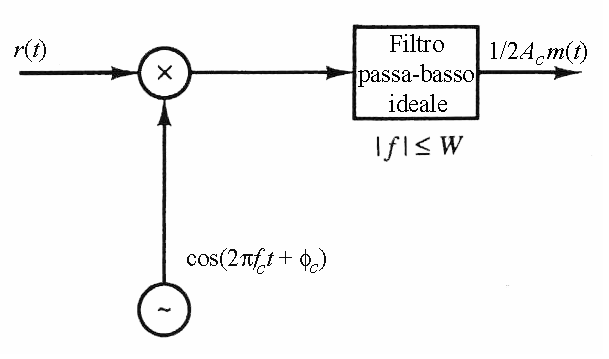
\includegraphics[scale = 1]{Schema architettura di un demodulatore.png}
\end{figure} 

dove avevamo nel caso DSB-SC: 

{
    \Large 
    \begin{equation}
        y_l (t)
        = 
        \frac{1}{2} A_c m(t) \cos(\phi_c - c)
    \end{equation}
}   

nel caso SSB in banda laterale superiore con $\phi_c = 0$, 
avremo che: 

{
    \Large 
    \begin{equation}
        \begin{split}
        u(t)
        &=
        A_c m(t) \cos(2 \pi f_c t)
        -
        A_c \tilde{m}(t) \sin(2 \pi f_c t) 
        \\
        &\downarrow
        \\
        y_l (t)
        &=
        \frac{1}{2} A_c m(t) \cos(\phi)
        + 
        \frac{1}{2} A_c \tilde{m}(t) \sin(\phi)
        \end{split}
    \end{equation}
}

Dalla formula di $y_l (t)$ notiamo che il segnale utile $\frac{1}{2} A_c m(t) \cos(\phi)$ 
è sovrapposto alla sua trasformata di Hilbert, che è ovviamente diversa dal segnale originale. \newline 

Ecco perché è importante realizzare un controllo molto accurato della fase $\phi$ al ricevitore (ad esempio impiegando i PLL), 
in modo da evitare che il problema evidenziato si presenti. \newline 

Per problema evidenziato della fase $\phi$ si intende che, nel caso peggiore in cui: 

{
    \Large 
    \begin{equation}
        \phi = 0^{\circ}
    \end{equation}
}

allora: 

{
    \Large 
    \begin{equation}
        \begin{split}
        y_l (t)
        &=
        \frac{1}{2} A_c m(t) \cos(\phi)
        + 
        \frac{1}{2} A_c \tilde{m}(t) \sin(\phi)
        \\
        &\downarrow
        \\
        y_l (t)
        &=
        \frac{1}{2} A_c m(t) \cos(0^{\circ})
        + 
        \frac{1}{2} A_c \tilde{m}(t) \sin(0^{\circ})
        \\
        &= 
        0
        +
        \frac{1}{2} A_c \tilde{m}(t)
        \\
        &= 
        \frac{1}{2} A_c \tilde{m}(t)
        \end{split}
    \end{equation}
}

cioè è presente solo la trasformata di Hilbert di m(t). \newline 

In modo da evitare questo problema, come ribadito nella DSB-SC, si può trasmettere un tono pilota a $f_c$, 
sprecando sulla potenza e sulla efficienza notevole della modulazione SSB. \newline 

\newpage 

\subsubsection{Modulazione di ampiezza con portanti in quadratura}
\footnote{Slide del prof | Modulazioni analogiche | pag 13 - 14\\  
Appunti di Damiano| pag 13 - 14\\
Appunti | Modulazioni analogiche | pag 13 - 14\\
Appunti | 2025-03-03 | pag 13 - 15
} 

A chiusura di questo sezione, vogliamo evidenziare che la medesima efficienza spettrale del segnale SSB 
può essere conseguita utilizzando due portanti in quadratura, alla stessa frequenza, 
a ciascuna delle quali sia associato un diverso segnale modulante. \newline 

La funzione del tempo che ne risulta può essere scritta come: 

{
    \Large 
    \begin{equation}
        u (t)
        = 
        A_c m_1 (t) \cos(2 \pi f_c t)
        + 
        A_c m_2 (t) \cos(2 \pi f_c t)
    \end{equation}
}

La seguente figura mostra a sinistra la generazione del segnale al lato trasmettitore, 
mentre a destra della figura si recupera $m_1 (t)$ e $m_2 (t)$ al lato ricevitore: 

\begin{figure}[h]
    \centering
    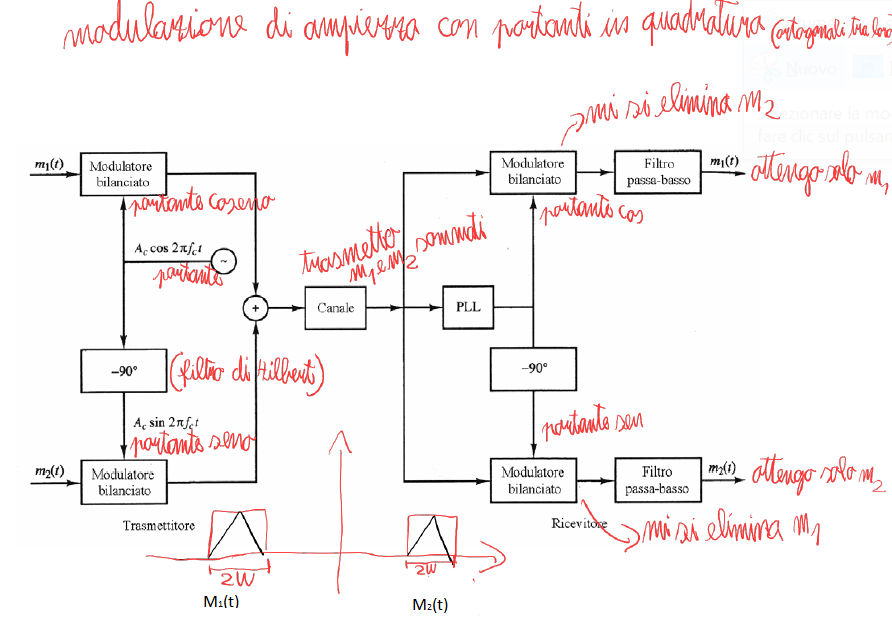
\includegraphics[scale = 1]{Schema con note di modulatore e demodulatore in quadratura.png}
\end{figure} 

Questo tipo di schema ci permette di dire che è possibile realizzare delle modulazioni DSB-SC che in ricezione è possibile separare, 
grazie alla ortogonalità delle portanti. \newline 

Pertanto, in questo caso, si pongono gli stessi problemi di ricostruzione della fase, 
e se ciò non avviene a dovere, il segnale, ad esempio $m_1(t)$, 
sarà sovrapposto a un residuo dell'altro segnale $m_2 (t)$: questa sovrapposizione è definita come cross-talk. \newline 

La modulazione di ampiezza con portanti in quadratura è l'archetipo di una delle modulazioni più importanti: 
la cosiddetta QAM Quadrature Amplitude Modulation, che avremo di approfondire nell'ambito delle modulazioni digitali. \newline 

\newpage 

\subsection{Banda laterale ridotta - VSB}
\footnote{Slide del prof | Modulazioni analogiche | pag 14 - 15\\  
Appunti di Damiano| pag 14 - 15\\
Appunti | Modulazioni analogiche | pag 14 - 15\\
Appunti | 2025-03-04 | pag 2 - 4\\ 
Appunti | 2025-07-08 Ricevimento | pag 10
} 

Per i segnali le cui caratteristiche spettrali non consentono l'utilizzo della modulazione SSB, 
si può migliorare l'efficienza spettrale utilizzando la modulazione di ampiezza a banda laterale ridotta 
(BLR in italiano, o in inglese VSB Vestigal Side Band). \newline 

\begin{tcolorbox}
Con la frase "i segnali le cui caratteristiche spettrali non consentono l'utilizzo della modulazione SSB" 
si intende che la SSB non è indicata per segnali che hanno una informazione significativa alle basse frequenze.  \newline

Letteralmente dall'inglese Vestigal significa residuo
\end{tcolorbox}

L'idea è quella di trasmettere un segnale che contenga una delle due bande laterali, ma anche una porzione (un vestiglio, un residuo) 
dell'altra banda laterale. \newline 

Il risultato è ottenuto con un opportuno filtraggio ad alta frequenza, come spiegato in questa figura: 

\begin{figure}[h]
    \centering
    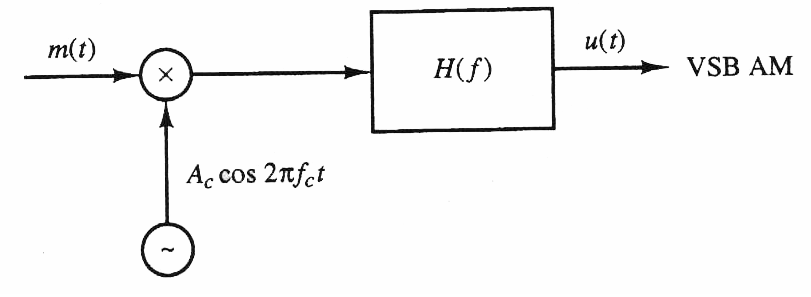
\includegraphics[scale = 0.8]{Architettura modulazione VSB.png}
\end{figure} 

Dallo schema notiamo che, nel tempo: 

{
    \Large 
    \begin{equation}
        u (t) 
        = 
        A_c m(t) \cos(2 \pi f_c t) 
        \otimes
        h(t)
    \end{equation}
}

dove: 

\begin{itemize}
    \item $A_c m(t) \cos(2 \pi f_c t)$ è il segnale modulato in DSB-SC
    \item il segno $\otimes$ indica la convoluzione 
    \item h(t) è la risposta impulsiva del filtro 
\end{itemize}

Dalle proprietà tra tempo e Fourier, sappiamo che, se facciamo una convoluzione nel tempo, avremo un prodotto in frequenza. \newline 

Quindi u(t) in Fourier diventa: 

{
    \Large 
    \begin{equation}
        \begin{split}
        u (t) 
        &= 
        A_c m(t) \cos(2 \pi f_c t) 
        \otimes
        h(t)
        \\
        U(f)
        &= 
        \frac{A_c}{2}
        \left[
            M(f - f_c) 
            +
            M(f + f_c)
        \right] 
        \cdot 
        H(f)
        \end{split}
    \end{equation}
}

Il filtro introduce massimo un'attenuazione di $\frac{1}{2}$: l'ampiezza della portante eventualmente trasmessa viene dimezzata. \newline 

Nelle applicazioni classiche della VSB (ad esempio al broadcasting televisivo), si utilizza la trasmissione della portante per semplificare il demodulatore, il quale può essere d'inviluppo. \newline 

Il filtro H(f) indicato in figura deve soddisfare la seguente condizione: 

{
    \Large 
    \begin{equation}
        H(f - f_c) 
        + 
        H(f + f_c)
        = 
        \text{ costante} 
    \end{equation}
}

Questa relazione deve essere valida per $\abs{f} \le W$. \newline 

Se questa relazione è soddisfatta, la demodulazione del segnale modulante, con banda W, avviene senza distorsione. \newline 

Come spiegato dalle seguenti figure: 

\begin{figure}[h]
    \centering
    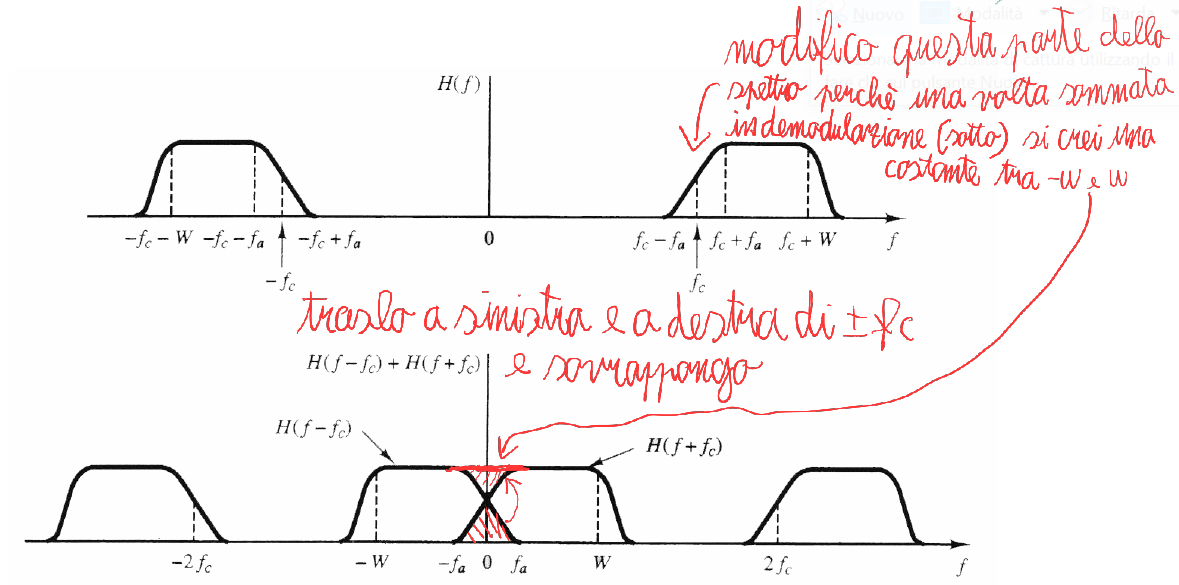
\includegraphics[scale = 0.6]{Grafici negli spettri da BB a modulato in VSB.PNG}
\end{figure} 

nella modulazione VSB, bisogna traslare una volta verso destra e una volta verso sinistra, della stessa quantità $f_c$, 
la funzione di trasferimento del filtro e di verificare che la somma delle due funzioni risultanti dalla due traslazione sia costante per $- W \le f \le +W$. \newline 

La banda occupata dal segnale VSB sarà di $W + f_a$, per cui il risparmio in banda può essere significativo. \newline 

De-modulando in modo coerente, consideriamo v(t) il segnale de-modulato nel tempo: 

{
    \Large 
    \begin{equation}
        v(t) = u(t) \cos(2 \pi f_c t)
    \end{equation}
}

In Fourier v(t) diventa: 

{
    \Large 
    \begin{equation}
        \begin{split}
           v(t) &= u^{'}(t) \cos(2 \pi f_c t)
           \\
           &\downarrow 
           \\
           V(f) &= \frac{1}{2} \left[ U(f - f_c) + U(f + f_c)\right] 
        \end{split}
    \end{equation}
}

Sostituendo il valore d U(f) a V(f), V(f) diventa: 

{
    \Large 
    \begin{equation}
        \begin{split}
             V(f) &= \frac{1}{2} \left[ U(f - f_c) + U(f + f_c)\right] 
             \\
             &\quad
             \\
             &\downarrow
             \\
             &\quad
             \\
             V(f) &= 
             \frac{A_c}{4} \left[ M(f- 2 f_c) + M(f)\right] \cdot H(f - f_c)
             +
            \frac{A_c}{4} \left[ M(f) + M(f + 2 f_c) \right] \cdot H(f + f_c)
        \end{split}
    \end{equation}
}

Riportando lo schema del demodulatore coerente: 

\begin{figure}[h]
    \centering
    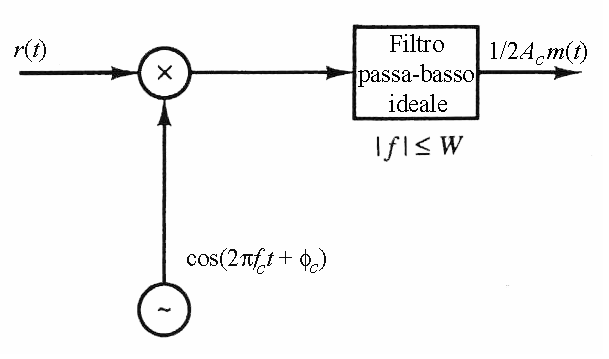
\includegraphics[scale = 1]{Schema architettura di un demodulatore.png}
\end{figure} 

i fattori $M(f- 2 f_c)$ e $M(f + 2 f_c)$ vengono eliminati, quindi V(f) si semplifica come: 

{
    \Large 
    \begin{equation}
        \begin{split}
             V(f) &= 
             \frac{A_c}{4} \left[ M(f- 2 f_c) + M(f)\right] \cdot H(f - f_c)
             +
            \frac{A_c}{4} \left[ M(f) + M(f + 2 f_c) \right] \cdot H(f + f_c)
            \\
            &\downarrow
            \\
            V(f) &= 
             \frac{A_c}{4} \left[ 0 + M(f)\right] \cdot H(f - f_c)
             +
            \frac{A_c}{4} \left[ M(f) + 0 \right] \cdot H(f + f_c)
            \\
            &= 
            \frac{A_c}{4} M(f) \left[ H(f - f_c) + H(f + f_c)\right]
        \end{split}
    \end{equation}
}

Siccome il nostro obbiettivo è recuperare M(f), cioè m(t), deve essere valida la relazione che abbiamo citato precedentemente: 

{
    \Large 
    \begin{equation}
        H(f - f_c) 
        + 
        H(f + f_c)
        = 
        \text{ costante} 
    \end{equation}
}

e per $\abs{f} \le W$. \newline 

\newpage 

\subsection{Altri schemi di modulatori di ampiezza}
\footnote{Slide del prof | Modulazioni analogiche | pag 15 - 18\\  
Appunti di Damiano| pag 15 - 18\\
Appunti | Modulazioni analogiche | pag 15 - 18\\
Appunti | 2025-03-04 | pag 5 - 7
} 

Oltre all'architetture delle modulazioni, è necessario fare qualche esempio riguardo la loro implementazione circuitale. \newline 

L'operazione di modulazione richiede, necessariamente, la presenza di componenti non lineari, 
i soli in grado di produrre le nuove frequenze richieste dalla conversione spettrale. \newline 

Un componente tipico è il diodo:  

\begin{figure}[h]
    \centering
    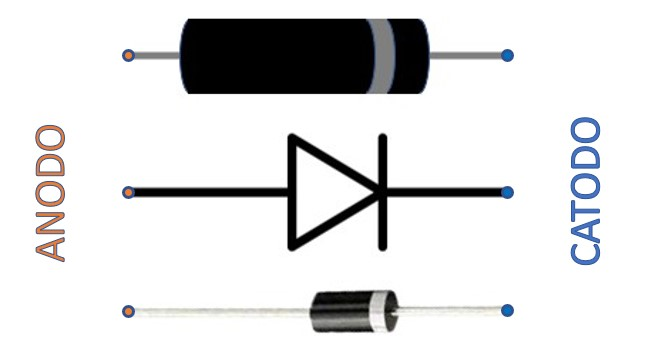
\includegraphics[scale = 0.4]{Diodo_come_funziona.jpg}
\end{figure} 

in cui la caratteristica funzione tensione-corrente ha questo tipo di andamento:

\begin{figure}[h]
    \centering
    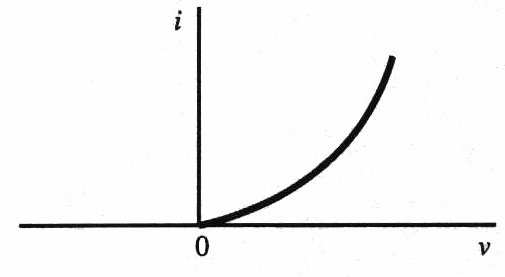
\includegraphics[scale = 0.6]{Grafico relazione tensione-corrente diodo.png}
\end{figure} 

In generale, è sufficiente la presenza di un elemento non lineare, 
la cui caratteristica ingresso-uscita presenti una componente quadratica. \newline 

Ragionando in tensione, ad esempio, deve aversi: 

{
    \Large 
    \begin{equation}
        v_0 (t)
        = 
        a_1 v_i (t)
        + 
        a_2 v_i^{2} (t)
    \end{equation}
}

in cui: 

\begin{itemize}
    \item $v_i (t)$ è il segnale in ingresso 
    \item $v_0 (t)$ è il segnale in uscita
\end{itemize}

Applicando in ingresso al dispositivo non lineare una funzione: 

{
    \Large
    \begin{equation}
        v_i (t)
        = 
        m(t) + A_c \cos(2 \pi f_c t)
    \end{equation}
} 

e filtrando con un filtro passa-banda centrato su $f_c$, come in figura: 

\begin{figure}[h]
    \centering
    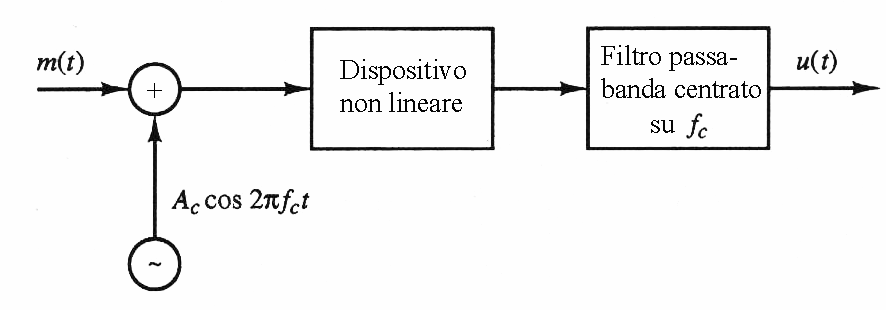
\includegraphics[scale = 0.6]{AM Convenzionale utilizzando un filtro passa-banda e un dipositivo non lineare.png}
\end{figure} 

l'uscita u(t) risulta, con le dovute semplificazioni: 

{
    \Large 
    \begin{equation}
        u(t)
        = 
        A_c a_1 \left[1 + \frac{2a_2}{a_1} m(t)\right] \cos(2 \pi f_c t)
    \end{equation}
}

u(t) ha le caratteristiche di un segnale modulato in ampiezza in modo convenzionale, 
i.e. AM convenzionale. \newline 

Inoltre, sapendo che u(t) è un segnale convenzionale, il termine $1 + \frac{2a_2}{a_1} m(t)$ non può essere negativo. \newline 

Grazie alla funzione caratteristica del diodo, che appunto è un dispositivo non lineare, 
è possibile realizzare uno "Switching Modulator", da cui si ottiene una modulazione AM-convenzionale, 
che ha il seguente schema circuitale: 

\begin{figure}[h]
    \centering
    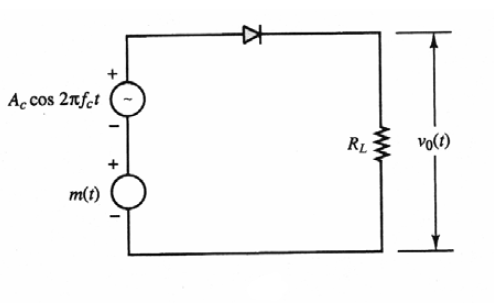
\includegraphics[scale = 1]{Switching Modulator schema circuitale.PNG}
\end{figure} 

oppure è possibile realizzare un "Ring Modulator", da cui si ottiene una modulazione DSB-SC, 
che ha il seguente schema circuitale: 

\begin{figure}[h]
    \centering
    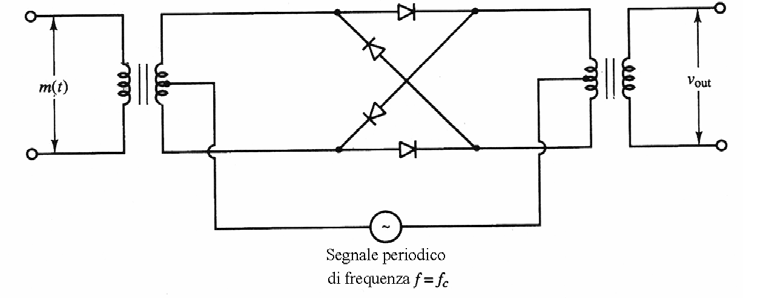
\includegraphics[scale = 1]{Ring Modulator schema circuitale.PNG}
\end{figure} 

Per lo schema dello "Switching Modulator" e del "Ring Modulator", 
il principio di funzionamento è quello di moltiplicare il segnale modulante m(t) per una funzione periodica p(t) di periodo $\frac{1}{f_c}$. \newline 

p(t), sviluppata in serie di Fourier, conterrà anche la componente di interesse a frequenza $f_c$. \newline 

Ad esempio l'uscita del circuito del Ring Modulator, che nel tempo ha questo andamento: 

\begin{figure}[h]
    \centering
    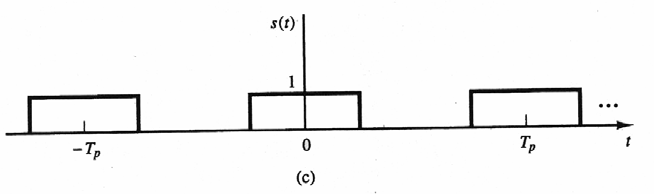
\includegraphics[scale = 1]{Andamento nel tempo tensione uscita Ring Modulator.png}
\end{figure} 


può essere scritta matematicamente come: 

{
    \Large 
    \begin{equation}
        \begin{split}
            v_0 (t) 
            &= 
            m(t) \cdot p(t)
            \\
            &= 
            m(t)
            \frac{4}{\pi} 
            \sum_{n = 1}^{+ \infty}
            \frac{(-1)^{n-1}}{2n - 1 }
            \cos [2 \pi f_c (2n - 1)]
        \end{split}
    \end{equation}
}

Come al solito, la componente di interesse può essere isolata utilizzando, a valle, un opportuno filtro passa-banda. \newline 

Un segnale DSB-SC può anche essere ottenuto combinando due modulatori identici AM convenzionali in uno schema bilanciato, come illustrato con la seguente figura: 

\begin{figure}[h]
    \centering
    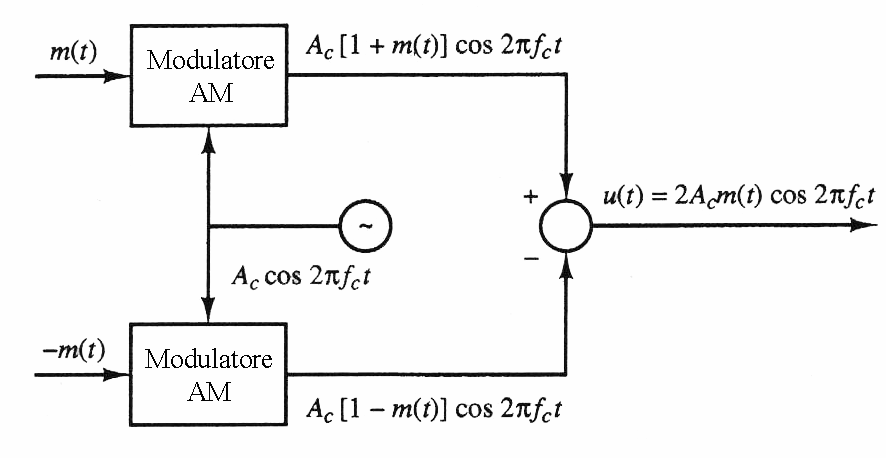
\includegraphics[scale = 0.8]{Architettura DSB-SC partendo da modulatori AM.png}
\end{figure} 

\begin{tcolorbox}
    Chiaraluce potrebbe tranquillamente, a mio parere, far insegnare un corso di Elettronica Analogica. Fine
\end{tcolorbox}

\newpage 

\section{Modulazione angolare}
\footnote{Slide del prof | Modulazioni analogiche | pag 18 - 21\\  
Appunti di Damiano| pag 18 - 21\\
Appunti | Modulazioni analogiche | pag 18 - 21\\
Appunti | 2025-03-04 | pag 8 - 9 \\
Appunti | 2025-03-07 | pag 2 
} 

Ricordando che un segnale c(t) (carrier, cioè segnale di portante) sinusoidale può essere descritto dalla seguente equazione: 

{
    \Large 
    \begin{equation}
        c(t) = A_c \cdot \cos(2 \pi f_c t + \phi_c)
    \end{equation}
}

il segnale della portante c(t) può, non solo modificare l'ampiezza del segnale modulante m(t), 
ma anche modificare la fase $\phi_c$ o la frequenza $f_c$. \newline 

In particolare, si parla di modulazione in fase PM (Phase Modulation) se il segnale modulato risulta: 

{
    \Large 
    \begin{equation}
        \begin{split}
            u(t)
            &= 
            A_c \cos(\theta (t))
            \\
            &= 
            A_c \cos(2 \pi f_c t + \phi(t))
        \end{split}
    \end{equation}
}

in cui: 

{
    \Large 
    \begin{equation}
        \phi (t) = k_p m(t)
    \end{equation}
}

dove $k_p$ è definito come costante di deviazione di fase. \newline 

Nella modulazione di fase, viene modificata $\phi$ in funzione del segnale modulante m(t) in maniera proporzionale. \newline 

Viene definita la frequenza istantanea del segnale u(t) come: 

{
    \Large 
    \begin{equation}
        \begin{split}
            f_i (t)
            &= 
            \frac{1}{2 \pi }
            \frac{d \theta(t)}{dt}
            \\
            &= 
            \frac{1}{2 \pi }
            \frac{d}{dt}
            (2 \pi f_c t + \phi (t))
            \\
            &= 
            f_c + f_c \frac{1}{2 \pi} \frac{d \phi (t)}{dt}
        \end{split}
    \end{equation}
}

$f_i (t)$ viene definita come modulazione di frequenza FM (Frequency Modulation) se risulta: 

{
    \Large 
    \begin{equation}
        f_i (t) - f_c = k_f m(t)
    \end{equation}
}

dove $k_f$ è definita come costante di deviazione di frequenza. \newline 

In altri termini, viene definita modulazione di frequenza quando la differenza rispetto a $f_c (t)$ è proporzionale a m(t) segnale modulante. \newline 

Se: 

{
    \Large 
    \begin{equation}
        m(t) = 0
    \end{equation}
}

nella modulazione di frequenza si trasmette solo $f_c(t)$, cioè la portante. \newline 

La modulazione FM e PM sono strettamente legate: 
dove esiste una esiste l'altra e viceversa. \newline 

In effetti. integrando l'espressione di $f_i (t)$ e tenendo conto dell'espressione di $k_f m(t)$, 
possiamo esprimere la fase $\phi (t)$ come: 

{
    \Large 
    \begin{equation}
        \phi (t)
        = 
        2 \pi k_f 
        \int_{- \infty}^{t}
        m (\tau) d\tau
    \end{equation}
}

A sua volta, derivando: 

{
    \Large 
    \begin{equation}
        \phi (t) = k_p m(t)
    \end{equation}
}

e tenendo conto dell'espressione di $f_i (t)$, 
si conclude che la PM è esprimibile come FM se: 

{
    \Large 
    \begin{equation}
        f_i (t) - f_c 
        =
        \frac{1}{2 \pi} k_p \frac{d}{dt} m(t)
    \end{equation}
}

In base a queste due espressioni, possiamo dire che la FM può essere vista come una PM in cui m(t) viene integrato, 
invece la PM può essere vista come una FM in cui m(t) viene derivata. \newline 

Ricapitolando si parla di FM o PM quando: 

{
    \Large 
    \begin{equation}
        \phi (t)
        = 
        \begin{cases}
            \begin{array}{ll}
            k_p m(t) & \textbf{ PM} 
            \\
            \\
            2 \pi k_f \int_{-\infty}^{t} m(\tau) d\tau & \textbf{ FM}
            \end{array} 
        \end{cases}
    \end{equation}
}

e 

{
    \Large 
    \begin{equation}
        f_i (t) - f_c
        = 
        \begin{cases}
            \begin{array}{ll}
            \frac{1}{2 \pi} k_p \frac{d}{dt} m(t) & \textbf{ PM} 
            \\
            \\
            k_f m(t) & \textbf{ FM}
            \end{array} 
        \end{cases}
    \end{equation}
}

Queste considerazioni danno un'indicazione esplicita su come realizzare il modulatore. \newline 

\newpage 

Come viene spiegato dalle seguenti figure: 

\begin{figure}[h]
    \centering
    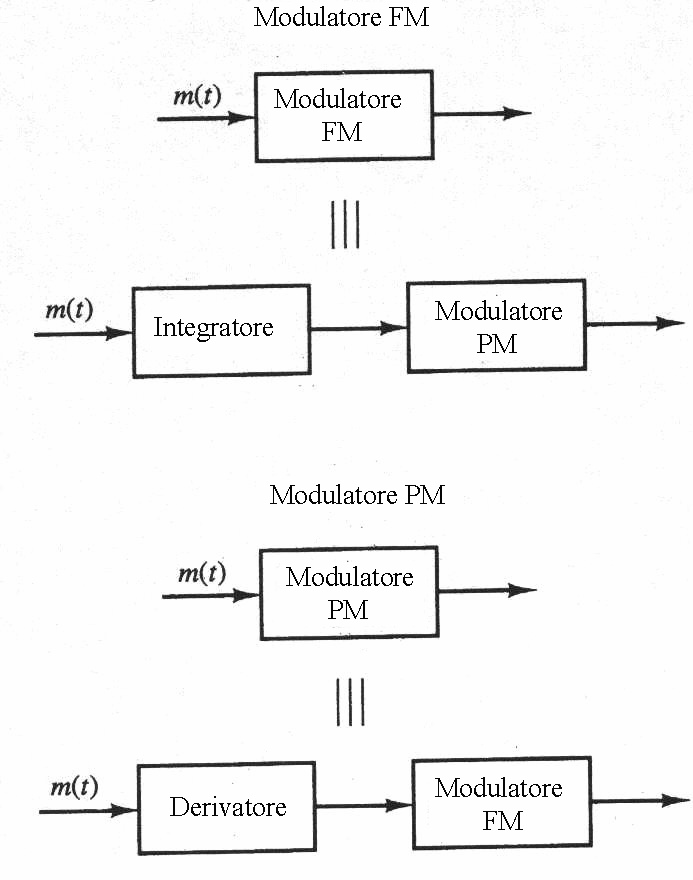
\includegraphics[scale = 0.8]{Modulatore FM e PM interscambiabili.png}
\end{figure} 

con l'aggiunta di un circuito o integratore o derivatore, 
è possibile realizzare un modulatore FM o PM partendo dal suo reciproco. \newline 

\newpage

Inoltre, visualizzando i segnali di ingresso e quelli di uscita dei modulatori: 

\begin{figure}[h]
    \centering
    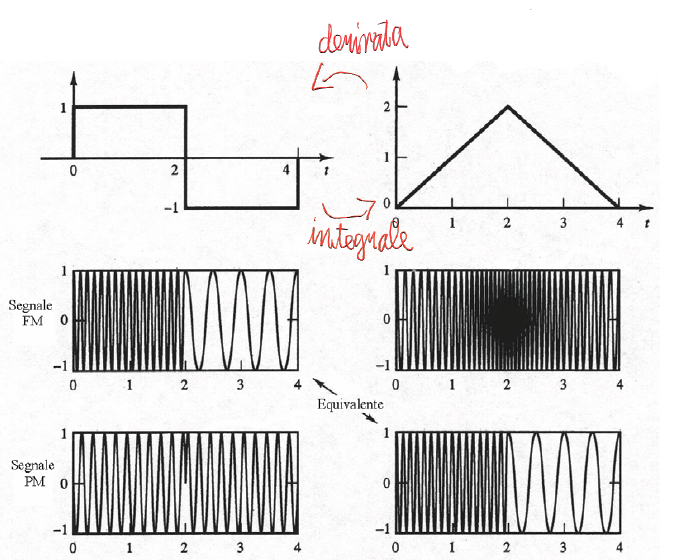
\includegraphics[scale = 1]{Andamenti segnali FM e PM.PNG}
\end{figure} 

possiamo osservare che i segnali FM e PM, con le osservazioni svolte, sono equivalenti. \newline 

Stabilita questa corrispondenza tra le due tecniche di modulazione, si può parlare genericamente di modulazione angolare. \newline 

\newpage 

\subsection{Indici della modulazione angolare}
\footnote{Slide del prof | Modulazioni analogiche | pag 21 - 23\\  
Appunti di Damiano| pag 21 - 23\\
Appunti | Modulazioni analogiche | pag 21 - 23\\
Appunti | 2025-03-07 | pag 2 - 3
} 

Per il fatto che il segnale modulante agisce sull'argomento della portante, 
la modulazione angolare è più difficile da trattare rispetto alla modulazione in ampiezza. \newline 

La modulazione di ampiezza è molto semplice: basta traslare lo spettro del segnale in BB a frequenza di portante. \newline 

Invece questo fatto, nelle angolazioni angolari, non avviene; alche la modulazione angolare è definita come modulazione non lineare, a differenza di quella di ampiezza. \newline 

Per questo motivo, molti dei calcoli relativi alla modulazione angolare sono stati preventivati considerando, 
come segnale modulante, il segnale sinusoidale. \newline 

Per una modulante sinusoidale: 

{
    \Large 
    \begin{equation}
        m(t) = a \cos(2 \pi f_m t)
    \end{equation}
}

si definisce come indici di modulazione, rispettivamente di fase $\beta_p$ e di frequenza $\beta_f$, come segue: 

{
    \Large 
    \begin{equation}
        \beta_p = k_p a
    \end{equation}
}

{
    \Large 
    \begin{equation}
        \beta_f = \frac{k_f a}{f_m}
    \end{equation}
}

Grazie a questi indici, possiamo esprimere il segnale modulato u(t) come: 

{
    \Large 
    \begin{equation}
        u(t)
        = 
        \begin{cases}
            \begin{array}{ll}
            A_c \cos \left[ 2 \pi f_c t + \beta_p \cos(2 \pi f_m t)\right] & \textbf{ PM} 
            \\
            A_c \cos \left[ 2 \pi f_c t + \beta_f \sin(2 \pi f_m t)\right] & \textbf{ FM}
            \end{array} 
        \end{cases}
    \end{equation}
}

È immediato verificare che $k_p a$ rappresenta la massima deviazione di fase $\Delta \phi_{max}$: 

{
    \Large 
    \begin{equation}
        \Delta \phi_{max}
        = 
        k_p \max \abs{m(t)}
    \end{equation}
}

nella PM. \newline 

Invece nella FM, $k_f a$ rappresenta la massima deviazione di frequenza $\Delta f_{max}$: 

{
    \Large 
    \begin{equation}
    \Delta f_{max}
        = 
        k_f \max \abs{m(t)}
    \end{equation}
} 

Grazie a queste definizioni, possiamo riscrivere $\beta_p$ e $\beta_f$ come: 

{
    \Large 
    \begin{equation}
        \beta_p = \Delta \phi_{max}
    \end{equation}
}

{
    \Large 
    \begin{equation}
        \beta_f = \frac{\Delta f_{max}}{f_m}
    \end{equation}
}

Originariamente introdotte per il caso di segnale modulante sinusoidale, 
le definizioni di $\beta_p$ e $\beta_f$ possono essere estese ad un segnale modulante qualsiasi, 
a patto di sostituire $f_m$ con la sua larghezza di banda W. \newline 

Formalmente, per la PM, per un segnale qualsiasi modulante di larghezza di banda W, rimane uguale a prima, quindi: 

{
    \Large 
    \begin{equation}
        \beta_p = \Delta \phi_{max}
    \end{equation}
}

invece, per la FM, diventa: 

{
    \Large 
    \begin{equation}
        \beta_f = \frac{\Delta f_{max}}{W}
    \end{equation}
}

Se un segnale avesse più frequenze, bisogna considerare la banda totale del segnale modulante W. \newline 

\newpage 


\subsubsection{Modulazione angolare a basso indice}
\footnote{Slide del prof | Modulazioni analogiche | pag 23 - 24\\  
Appunti di Damiano| pag 23 - 24\\
Appunti | Modulazioni analogiche | pag 23 - 24\\
Appunti | 2025-03-07 | pag 3 - 4\\
Appunti | 2025-07-08 Ricevimento | pag 10
} 

L'indice di modulazione $\beta$ è un parametro fondamentale della modulazione angolare 
e svolge un ruolo chiave nella qualità di trasmissione quando il segnale è affetto da rumore. \newline 

Si parla di modulazione angolare a basso indice (o modulazione angolare a banda stretta)
quando la variazione di $\phi (t)$: 

{
    \Large 
    \begin{equation}
        \phi (t)
        = 
        \begin{cases}
            \begin{array}{ll}
            k_p m(t) & \textbf{ PM} 
            \\
            \\
            2 \pi k_f \int_{-\infty}^{t} m(\tau) d\tau & \textbf{ FM}
            \end{array} 
        \end{cases}
    \end{equation}
}

risulta molto piccola, cioè: 

{
    \Large 
    \begin{equation}
        \phi (t) << 1
    \end{equation}
}

Sotto questa ipotesi, il segnale modulato con modulazione angolare da: 

{
    \Large 
    \begin{equation}
        \begin{split}
            u(t)
            &= 
            A_c \cos(\theta (t))
            \\
            &= 
            A_c \cos(2 \pi f_c t + \phi(t))
        \end{split}
    \end{equation}
}

diventa: 

{
    \Large
    \begin{equation}
        \begin{split}
        u(t)
        &= 
        A_c \cos(2 \pi f_c t + \phi (t))   
        \\
        &= 
        A_c \cos(2\pi f_c t) \cos(\phi (t)) 
        - 
        A_c \sin(2\pi f_c t) \sin(\phi (t))
        \\
        &\approx
        A_c \cos(2\pi f_c t)  
        - 
        A_c \sin(2\pi f_c t) \phi (t)
        \\
        &= 
        A_c \cos(2\pi f_c t)  
        - 
        A_c \phi (t) \sin(2\pi f_c t) 
    \end{split}
    \end{equation}
}

\begin{tcolorbox}
Non dobbiamo impararci le formule a memoria. \newline 

Dobbiamo solo sapere che l'informazione è contenuta nella fase $\phi (t)$. \newline

    Dall'analisi matematica 1, 
    si è potuto approssimare $\sin(\phi(t))$ a $\phi (t)$ grazie alla teoria degli o-piccoli. \newline 

    Ripassino al volo che non fa mai male: \\
    \url{https://www.youmath.it/lezioni/analisi-matematica/limiti-continuita-e-asintoti/3247-o-piccolo.html}
\end{tcolorbox}

Questa espressione di u(t) esplicita la somiglianza con l'espressione di un segnale modulato in AM convenzionale: 

{
    \Large 
    \begin{equation} 
        \begin{split}
        u (t)
        &= 
        A_c 
        [1 + \alpha \cdot m_n (t)] 
        \cos(2 \pi f_c t + \phi_c)
        \\
        &= 
        A_c \cos(2 \pi f_c t + \phi_c)
        +
        A_c \alpha \cdot m_n (t) \cos(2 \pi f_c t + \phi_c)
        \end{split}
    \end{equation}
}

\newpage 

Utilizzando il piano dei fasori, 
possiamo graficare le due espressione di u(t): 

\begin{figure}[h]
    \centering
    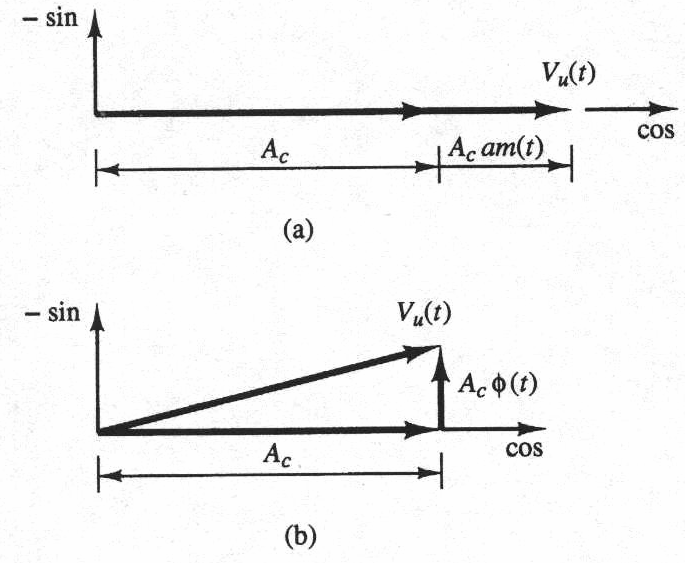
\includegraphics[scale = 1]{Confronto nel piano fasoriale tra AM e modulazione angolare a basso indice.png}
\end{figure} 

dove la prima in alto è u(t) con modulazione AM-convenzionale, 
invece la seconda in basso è u(t) con modulazione angolare a basso indice. \newline 

Si può svolgere la seguente osservazione: 
nella AM convenzionale, il modulo di $V_u (t)$ varia in base alla modulazione (vedo m(t) che si trova sul piano del coseno) e il suo angolo rimane costante; 
invece, nella modulazione angolare, abbiamo che il modulo di $V_u (t)$ rimane costate, ma varia il suo angolo (vedi $\phi (t)$ sul piano del seno). \newline 

Per fissare bene le idee, consideriamo al caso PM in cui il segnale modulato vale: 

{
    \Large 
    \begin{equation}
        u(t) 
        \approx
        A_c \cos(2 \pi f_c t)
        - 
        A_c k_p m(t) \sin(2 \pi f_c t) 
    \end{equation}
}

Facendo la trasformata di Fourier di u(t) e considerando m(t) reale pari, sapendo le proprietà tra trasformata di Fourier nel tempo e in frequenza anche M(f) sarà a sua volta reale pari, 
possiamo visualizzare U(f) come: 

\begin{figure}[h]
    \centering
    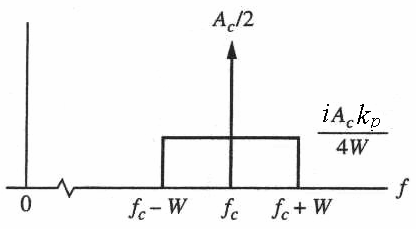
\includegraphics[scale = 1]{Segnale PM modulato a basso indice in Fourier.png}
\end{figure} 

dove in figura si considerano solo le frequenze positive. \newline 

Si parla di modulazione angolare a banda stretta perché, come si visualizza in figura, 2W è la minima occupazione 
spettrale conseguibile in modulazione angolare, quindi PM e FM, e si ottiene sono nell'ipotesi di: 

{
    \Large 
    \begin{equation}
        \phi (t) << 1
    \end{equation}
}

\newpage 

\subsection{Banda di una modulazione angolare}
\footnote{Slide del prof | Modulazioni analogiche | pag 25 - 26\\  
Appunti di Damiano| pag 25 - 26\\
Appunti | Modulazioni analogiche | pag 25 - 26\\
Appunti | 2025-03-07 | pag 4
} 

Assumendo per il segnale modulante m(t) una funzione cosinusoidale con frequenza $f_m$, 
si può scrivere: 

{
    \Large 
    \begin{equation}
        u(t) 
        = 
        A_c 
        \cos(2 \pi f_c t + \beta \cos(2 \pi f_m t))
    \end{equation}
}

con $\beta = \beta_p$ se si fa una PM o $\beta = \beta_f$ se si fa una FM. \newline 

Visto che analiticamente è difficile svolgere un coseno dentro ad un coseno, 
u(t) può essere riscritta come: 

{
    \Large 
    \begin{equation}
        u(t)
        = 
        \sum_{n = -\infty}^{+ \infty}
        A_c 
        J_n (\beta) \cos \left[ 2 \pi (f_c + n f_m) t\right]
    \end{equation}
}

dove $J_n (\beta)$ è la funzione di Bessel di prima specie di ordine n. \newline 

\begin{tcolorbox}
    Cosa sono e perché si utilizzano in casi particolari le funzioni di Bessel? \newline 

    \url{https://it.wikipedia.org/wiki/Equazioni_di_Bessel}
\end{tcolorbox}

Alcuni andamenti di $J_n (\beta)$: 

\begin{figure}[h]
    \centering
    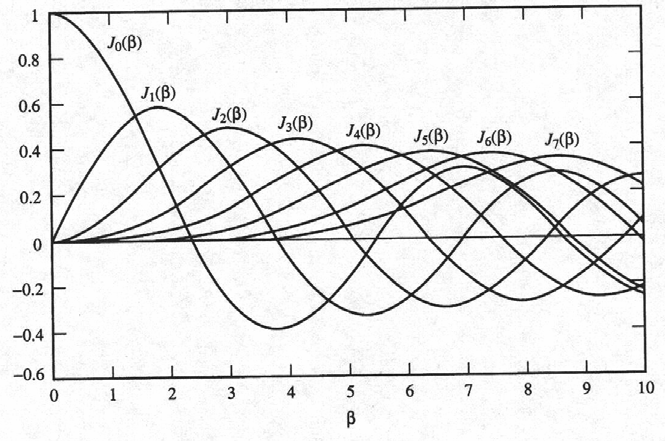
\includegraphics[scale = 1]{Funzioni di Bessel.png}
\end{figure}

Sulla base della formula di u(t), notiamo che u(t) è esprimibile con una sommatoria di infiniti termini, 
in cui avremo, nello spettro, infinite armoniche, quindi infinite righe ogni frequenza multipla di $f_m$. \newline 

Per questo motivo la modulazione angolare non viene definita lineare come la modulazione in ampiezza, 
perché, in questo caso, lo spettro in BB non viene semplicemente traslato alla frequenza della portante. \newline 

Inoltre, sapendo che la potenza del segnale modulato è costante a pari a $\frac{A_c ^{2}}{2}$ (dalle proprietà di ciclo-stazionarietà dello spettro in frequenza), 
si può dire che la potenza delle funzioni di Bessel vale: 

{
    \Large 
    \begin{equation}
        \sum_{n = - \infty}^{+ \infty}
        \left[ J_n (\beta)\right]^{2} = 1
    \end{equation}
}

Questa è una proprietà delle funzioni di Bessel di prima specie. \newline 

L'occupazione illimitata della banda non consentirebbe un utilizzo pratico del sistema. \newline 

Se però si visualizza l'andamento delle funzioni di Bessel, si nota che, per ogni valore di $\beta$, 
c'è un numero limitato di funzioni di Bessel che danno un contributo significativo. \newline 

In particolare, risulta applicabile la regola secondo cui le funzioni di Bessel di ordine n: 

{
    \Large 
    \begin{equation}
        n \le \beta + 1
    \end{equation}
}

sono apprezzabilmente diverse da zero. \newline 

Invece le funzioni di Bessel di ordine n: 
{
    \Large 
    \begin{equation}
        n > \beta + 1
    \end{equation}
} 

sono trascurabili. \newline 

Sulla base di queste considerazioni, si può concludere che delle infinite armoniche nominalmente presenti nello spettro del segnale modulato 
danno, in realtà, contributo significativo allo spettro solo quelle che distano dalla portante non più di $(\beta + 1)$ volte $f_m$. \newline 

Tenendo conto della distribuzione bilatera rispetto alla portante, ne risulta una banda "effettiva" occupata dalla modulazioni angolari di: 

{
    \Large 
    \begin{equation}
        B_c = 2 (\beta + 1) f_m
    \end{equation}
}

$B_c$ contiene il 98 \% della potenza totale del segnale. \newline 

Sapendo la relazione tra $\beta$ e $B_c$, possiamo esprimere $B_c$ per le due modulazioni angolari studiate: 

{
    \Large 
    \begin{equation}
        B_c
        = 
        \begin{cases}
            \begin{array}{ll}
            2 (k_p a + 1) f_m & \textbf{ PM} 
            \\
            2 (k_f a + f_m) & \textbf{ FM}
            \end{array} 
        \end{cases}
    \end{equation}
}

dove a è l'ampiezza del segnale modulante. \newline 

Da queste due formule di $B_c$ per PM e FM si nota che all'aumentare di a, aumenta $B_c$ sia nella PM che nella FM. \newline 

Invece, $f_m$ nella PM moltiplica il termine $2(k_p a + 1)$, 
invece nella FM, $f_m$ ha un ruolo additivo al termine $k_f a$. \newline 

Quindi, all'aumentare di $f_m$, la banda $B_c$ aumenta nettamente di più nella PM rispetto alla FM. \newline 

Queste formule della banda $B_c$ sono valide per un segnale modulante cosinusoidale. \newline 

\newpage

\subsubsection{Banda di una modulazione angolare per un segnale modulante qualsiasi}
\footnote{Slide del prof | Modulazioni analogiche | pag 26 - 27\\  
Appunti di Damiano| pag 26 - 27\\
Appunti | Modulazioni analogiche | pag 26 - 27\\
Appunti | 2025-03-07 | pag 4 - 5
}

Nel caso in cui si considera un generico segnale periodico (che possiamo generalizzare come caso di modulante cosinusoidale) 
e un processo gaussiano (esemplificativo di una funzione stocastica), si possono adattare i parametri visti precedente a questo caso. \newline 

La formula di $B_c$ vista precedentemente è valida se a $f_m$ si sostituisce la frequenza massima significativa W dello spettro del segnale modulante:
: 

{
    \Large 
    \begin{equation}
        \begin{split}
        B_c
        &= 
        \begin{cases}
            \begin{array}{ll}
            2 (k_p a + 1) f_m & \textbf{ PM} 
            \\
            2 (k_f a + f_m) & \textbf{ FM}
            \end{array} 
        \end{cases}
        \\
        &\downarrow
        \\
        B_c
        &= 
        \begin{cases}
            \begin{array}{ll}
            2 (k_p a + 1) W & \textbf{ PM} 
            \\
            2 (k_f a + W) & \textbf{ FM}
            \end{array} 
        \end{cases} 
        \end{split}
    \end{equation}
}


Lo stesso principio vale per l'altra formula di $B_c$: 

{
    \Large 
    \begin{equation}
        \begin{split}
            B_c &= 2 (\beta + 1) f_m 
        \\
        &\downarrow
        \\
        B_c &= 2 (\beta + 1) W
        \end{split}
    \end{equation}
}

Queste formula di $B_c$ costituisce una eccellente approssimazione della banda occupata da un segnale in modulazione angolare. \newline 

Questa formula è universalmente nota come "regola di Carson". \newline 

Ma, è bene precisare che, la formula di Carson nel caso FM, così calcolata, è una sottostima di $B_c$ se il valore di $\beta$ 
è compreso tra 2 e 10. \newline 

Quindi la formula di Carson, in questo caso particolare diventa: 

{
    \Large 
    \begin{equation}
        B_c = 2 (\beta_f + 2 ) W \textbf{ FM per  $ 2 < \beta_f < 10$ }
    \end{equation}
}

\newpage 

\subsection{Mo/demodulatori angolari}
\footnote{Slide del prof | Modulazioni analogiche | pag 27 - 31\\  
Appunti di Damiano| pag 27 - 31\\
Appunti | Modulazioni analogiche | pag 27 - 31\\
Appunti | 2025-03-10 | pag 2 - 4\\ 
Appunti | 2025-07-08 Ricevimento | pag 10
} 

Dalla formula della modulazione angolare PM a basso indice u(t): 

{
    \Large 
    \begin{equation}
        u(t) 
        \approx
        A_c \cos(2 \pi f_c t)
        - 
        A_c k_p m(t) \sin(2 \pi f_c t) 
    \end{equation}
}

possiamo dire che la modulazione angolare può essere vista come una modulazione AM-convenzionale con uno shift di $90^{\circ}$
(il seno rispetto al coseno differiscono di $90^{\circ}$) della portante. \newline 

Grazie a questa osservazione, possiamo costruire il seguente schema del modulatore angolare: 

\begin{figure}[h]
    \centering
    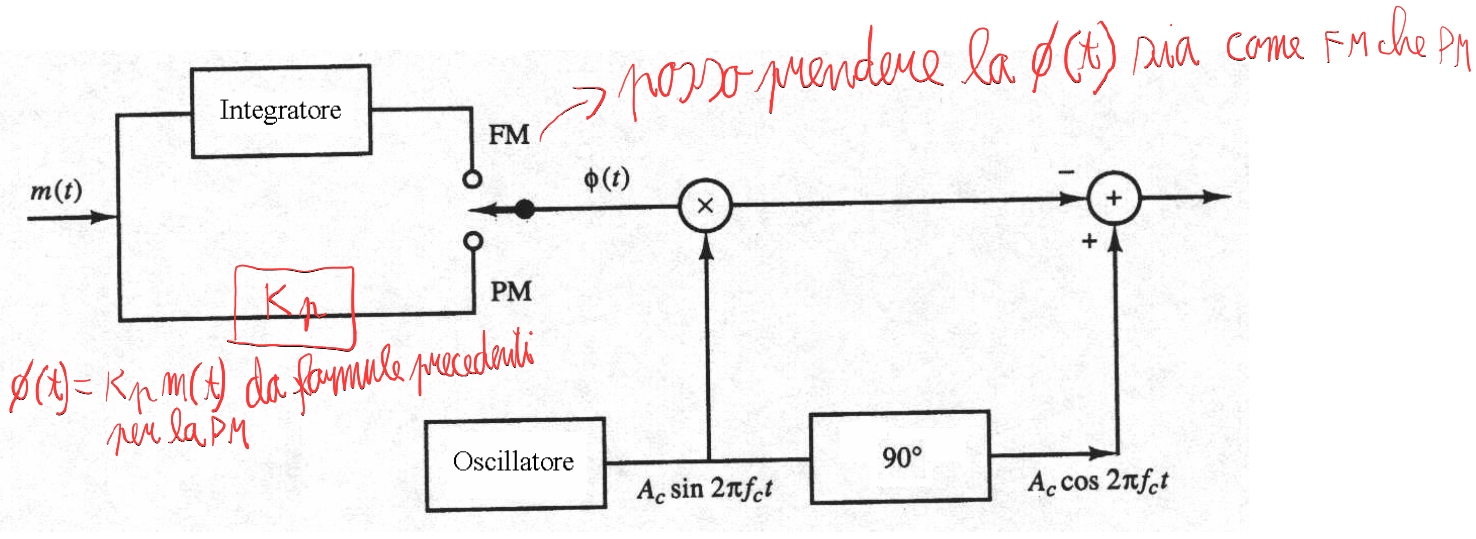
\includegraphics[scale = 0.6]{Modulatore di Armstrong.PNG}
\end{figure}

Questo tipo di modulatore angolare è definito come modulatore di Armstrong. \newline 

Invece, per un segnale FM, non necessariamente a basso indice, si ottiene utilizzando un diodo varactor o chiamato anche oscillatore in tensione (VCO: Voltage Controlled Oscillator). \newline 

Un possibile circuito per modulare un segnale FM a basso indice: 

\begin{figure}[h]
    \centering
    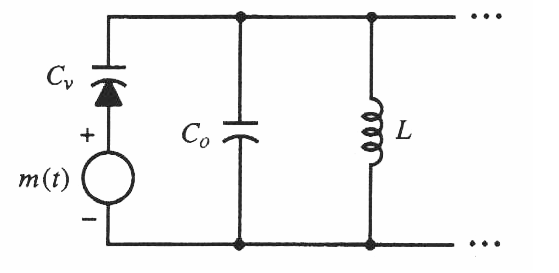
\includegraphics[scale = 0.8]{VCO.png}
\end{figure}

\begin{tcolorbox}
Quel componente segnato come $C_v$ che sembra sia un diodo che una capacità è un capacitore variabile che cambia il suo valore di capacità in base alla tensione ai suoi capi, 
in questo circuito $C_v$ cambia la sua capacità in base alla tensione di m(t) 
\end{tcolorbox}

Un altro circuito per generare un segnale FM o PM con indice di modulazione $\beta$ generico 
è quello del narrowband angle modulator, che fa riferimento al modulatore di Armstrong ma a banda stretta. \newline 

\newpage 

Di seguito, il disegno dell'architettura: 

\begin{figure}[h]
    \centering
    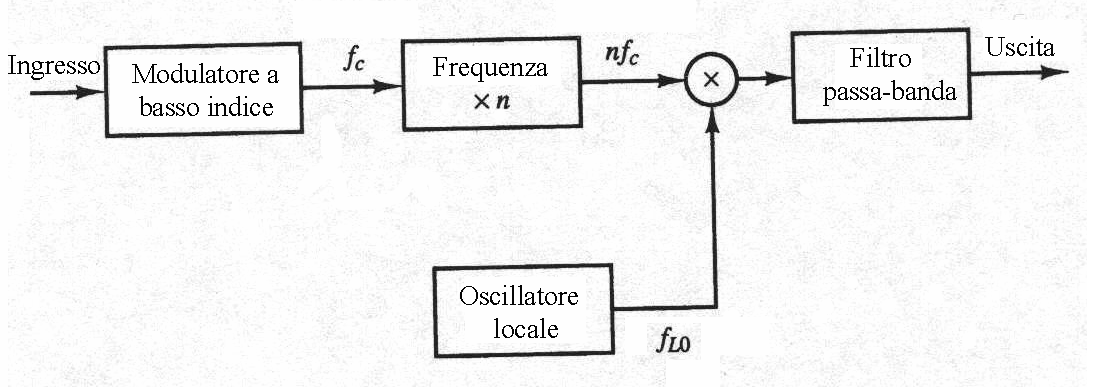
\includegraphics[scale = 0.8]{Narrowband angle modulator architettura.png}
\end{figure}

L'introduzione dell'oscillatore locale a frequenza $f_{LO}$ è dovuta alla necessità di allocare il segnale trasmesso alla frequenza di portante desiderata, 
ove tale non fosse il risultato della moltiplicazione di $n \cdot f_c$. \newline 

L'oscillatore locale serve per una conversione in frequenza. \newline 

Il filtro passa-banda toglie tutte le componenti che non sono necessarie. \newline 

La tecnica che applica questo tipo di architettura circuitale prende il nome di metodo indiretto. \newline 

\newpage 

\subsubsection{Demodulatori angolari}
\footnote{Slide del prof | Modulazioni analogiche | pag 28 \\  
Appunti di Damiano| pag 28 \\
Appunti | 2025-03-10 | pag 2 \\
Appunti | 2025-07-08 Ricevimento | pag 9
} 

Benché, in linea di principio, la demodulazione di un segnale PM o FM possa essere realizzata con tecniche coerenti (quindi moltiplicando per delle funzioni cosinusoidali), 
in grado di estrarre la fase del segnale (in cui è associata l'informazione), 
in pratica si preferisce di adottare tecniche non coerenti, in modo da semplificare drasticamente la struttura del ricevitore. \newline 

Consideriamo il caso solo della demodulazione in FM, sapendo che il demodulatore FM può essere anche un demodulatore PM. \newline 

L'idea è quella di convertire il segnale FM in segnale AM-convenzionale prima di procedere alla demodulazione. \newline 

Lo schema del demodulatore FM è il seguente: 

\begin{figure}[h]
    \centering
    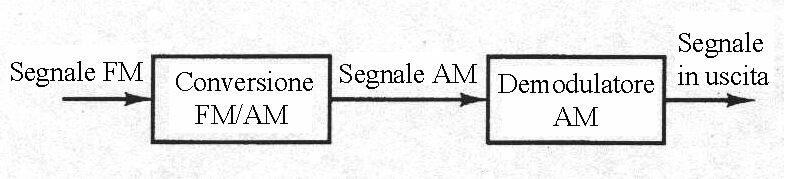
\includegraphics[scale = 0.8]{Demodulatore FM.png}
\end{figure}

in cui il convertitore FM/AM è un banale derivatore. \newline 

Ora andiamo a calcolare analiticamente la demodulazione. \newline 

Un possibile schema di un convertitore FM/AM: 

\begin{figure}[h]
    \centering
    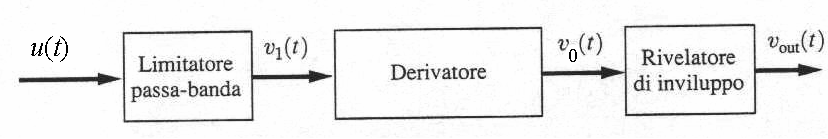
\includegraphics[scale = 0.8]{Convertitore FM-AM.png}
\end{figure}

Consideriamo il segnale in ingresso u(t) modulato: 

{
    \Large 
    \begin{equation}
        u(t)
        = 
        A_c 
        \cos 
        \left(
            2 \pi f_c t 
            + 
            2 \pi k_f \int_{- \infty}^{t} m(\tau) d\tau
        \right)
    \end{equation}
}

La funzione di trasferimento H(f) di un blocco derivatore è caratterizzato dalle seguente funzione: 

{
    \Large
    \begin{equation}
        \abs{H(f)} = V_0 + k(f - f_c) \textbf{ per } \abs{f - f_c} \le \frac{B_c}{2}
    \end{equation}
}

\begin{tcolorbox}
Dalle relazioni tra dominio del tempo e frequenza, 
una derivata nel tempo, dobbiamo avere un funzione lineare nell'intorno della frequenza da considerare, 
in questo caso nell'intorno di $f_c$. \newline 

Per realizzare questo filtro derivatore, si usano dei circuiti risonanti e si trova il loro tratto lineare. \newline 

Essendo circuiti risonanti composti da induttori, questi permettono di svolgere delle derivate nel tempo, 
grazie alla loro funzione caratteristica. 
\end{tcolorbox}

Per il resto, si tratta di una funzione puramente immaginaria, e dunque asimmetrica rispetto all'origine. \newline 

Il segnale che esce fuori dopo il filtro è: 

{
    \Large 
    \begin{equation}
        v_0 (t)
        = 
        - A_c 
        \left[
            V_0 + k k_f m(t)
        \right]
        \sin 
        \left(
            2 \pi f_c t 
            + 
            2 \pi k_f 
            \int_{-\infty}^{t} m(\tau) d\tau
        \right)
    \end{equation}
}

Il rivelatore di inviluppo estrae dalla funzione di $v_0 (t)$ l'argomento $- A_c 
        \left[
            V_0 + k k_f m(t)
        \right]$

\newpage



